\documentclass[aspectratio=169, 10pt]{beamer}
\usepackage{graphicx}
\usepackage{booktabs}
\usepackage{tikz}

% --- Theme & Colors ---
\usetheme{default}
\usefonttheme{structurebold}

% Custom Colors (Sumer-ish / NFL Front Office)
\definecolor{DarkBlue}{RGB}{20, 30, 60}
\definecolor{AccentGold}{RGB}{200, 160, 50}
\definecolor{LightGray}{RGB}{240, 240, 240}

\setbeamercolor{background canvas}{bg=white}
\setbeamercolor{frametitle}{fg=white, bg=DarkBlue}
\setbeamercolor{title}{fg=DarkBlue}
\setbeamercolor{structure}{fg=DarkBlue}
\setbeamercolor{item}{fg=AccentGold}

% Clean Footer
\setbeamertemplate{footline}[frame number]
\setbeamertemplate{navigation symbols}{}

% --- Metadata ---
\title{\huge \textbf{Separation Science}}
\subtitle{\large Contextual Separation Grades for Shrine Bowl WRs \& DBs}
\author{\textbf{Shrine Bowl Analytics 2026}}
\date{}

\begin{document}

% Slide 1: Title
\begin{frame}
    \begin{center}
        \vspace{-0.5cm} % Pull image up
        
\includegraphics[width=0.3\textwidth]{viz_logo_placeholder.png}
        \vspace{0.2cm}
    \end{center}
    \titlepage
\end{frame}

% Slide 2: The Challenge (Exec Summary)
\begin{frame}{1. The Challenge: Quantifying "Process Wins"}
    \begin{columns}
        \column{0.6\textwidth}
        \textbf{The Problem:}
        \begin{itemize}
            \item Scouts look for "stickiness" and "late separation," but eye tests are subjective.
            \item Box scores (catches/yards) ignore the 90\% of reps where the ball doesn't go their way.
        \end{itemize}
        
        \vspace{0.5cm}
        \textbf{Our Solution:}
        \begin{itemize}
            \item \textbf{Separation Efficiency:} A physics-based grade for every route cut (N=246 reps).
            \item \textbf{WROE:} "Win Rate Over Expected" - Context-aware grading (The Moneyball Metric).
        \end{itemize}

        \column{0.4\textwidth}
        \centering
        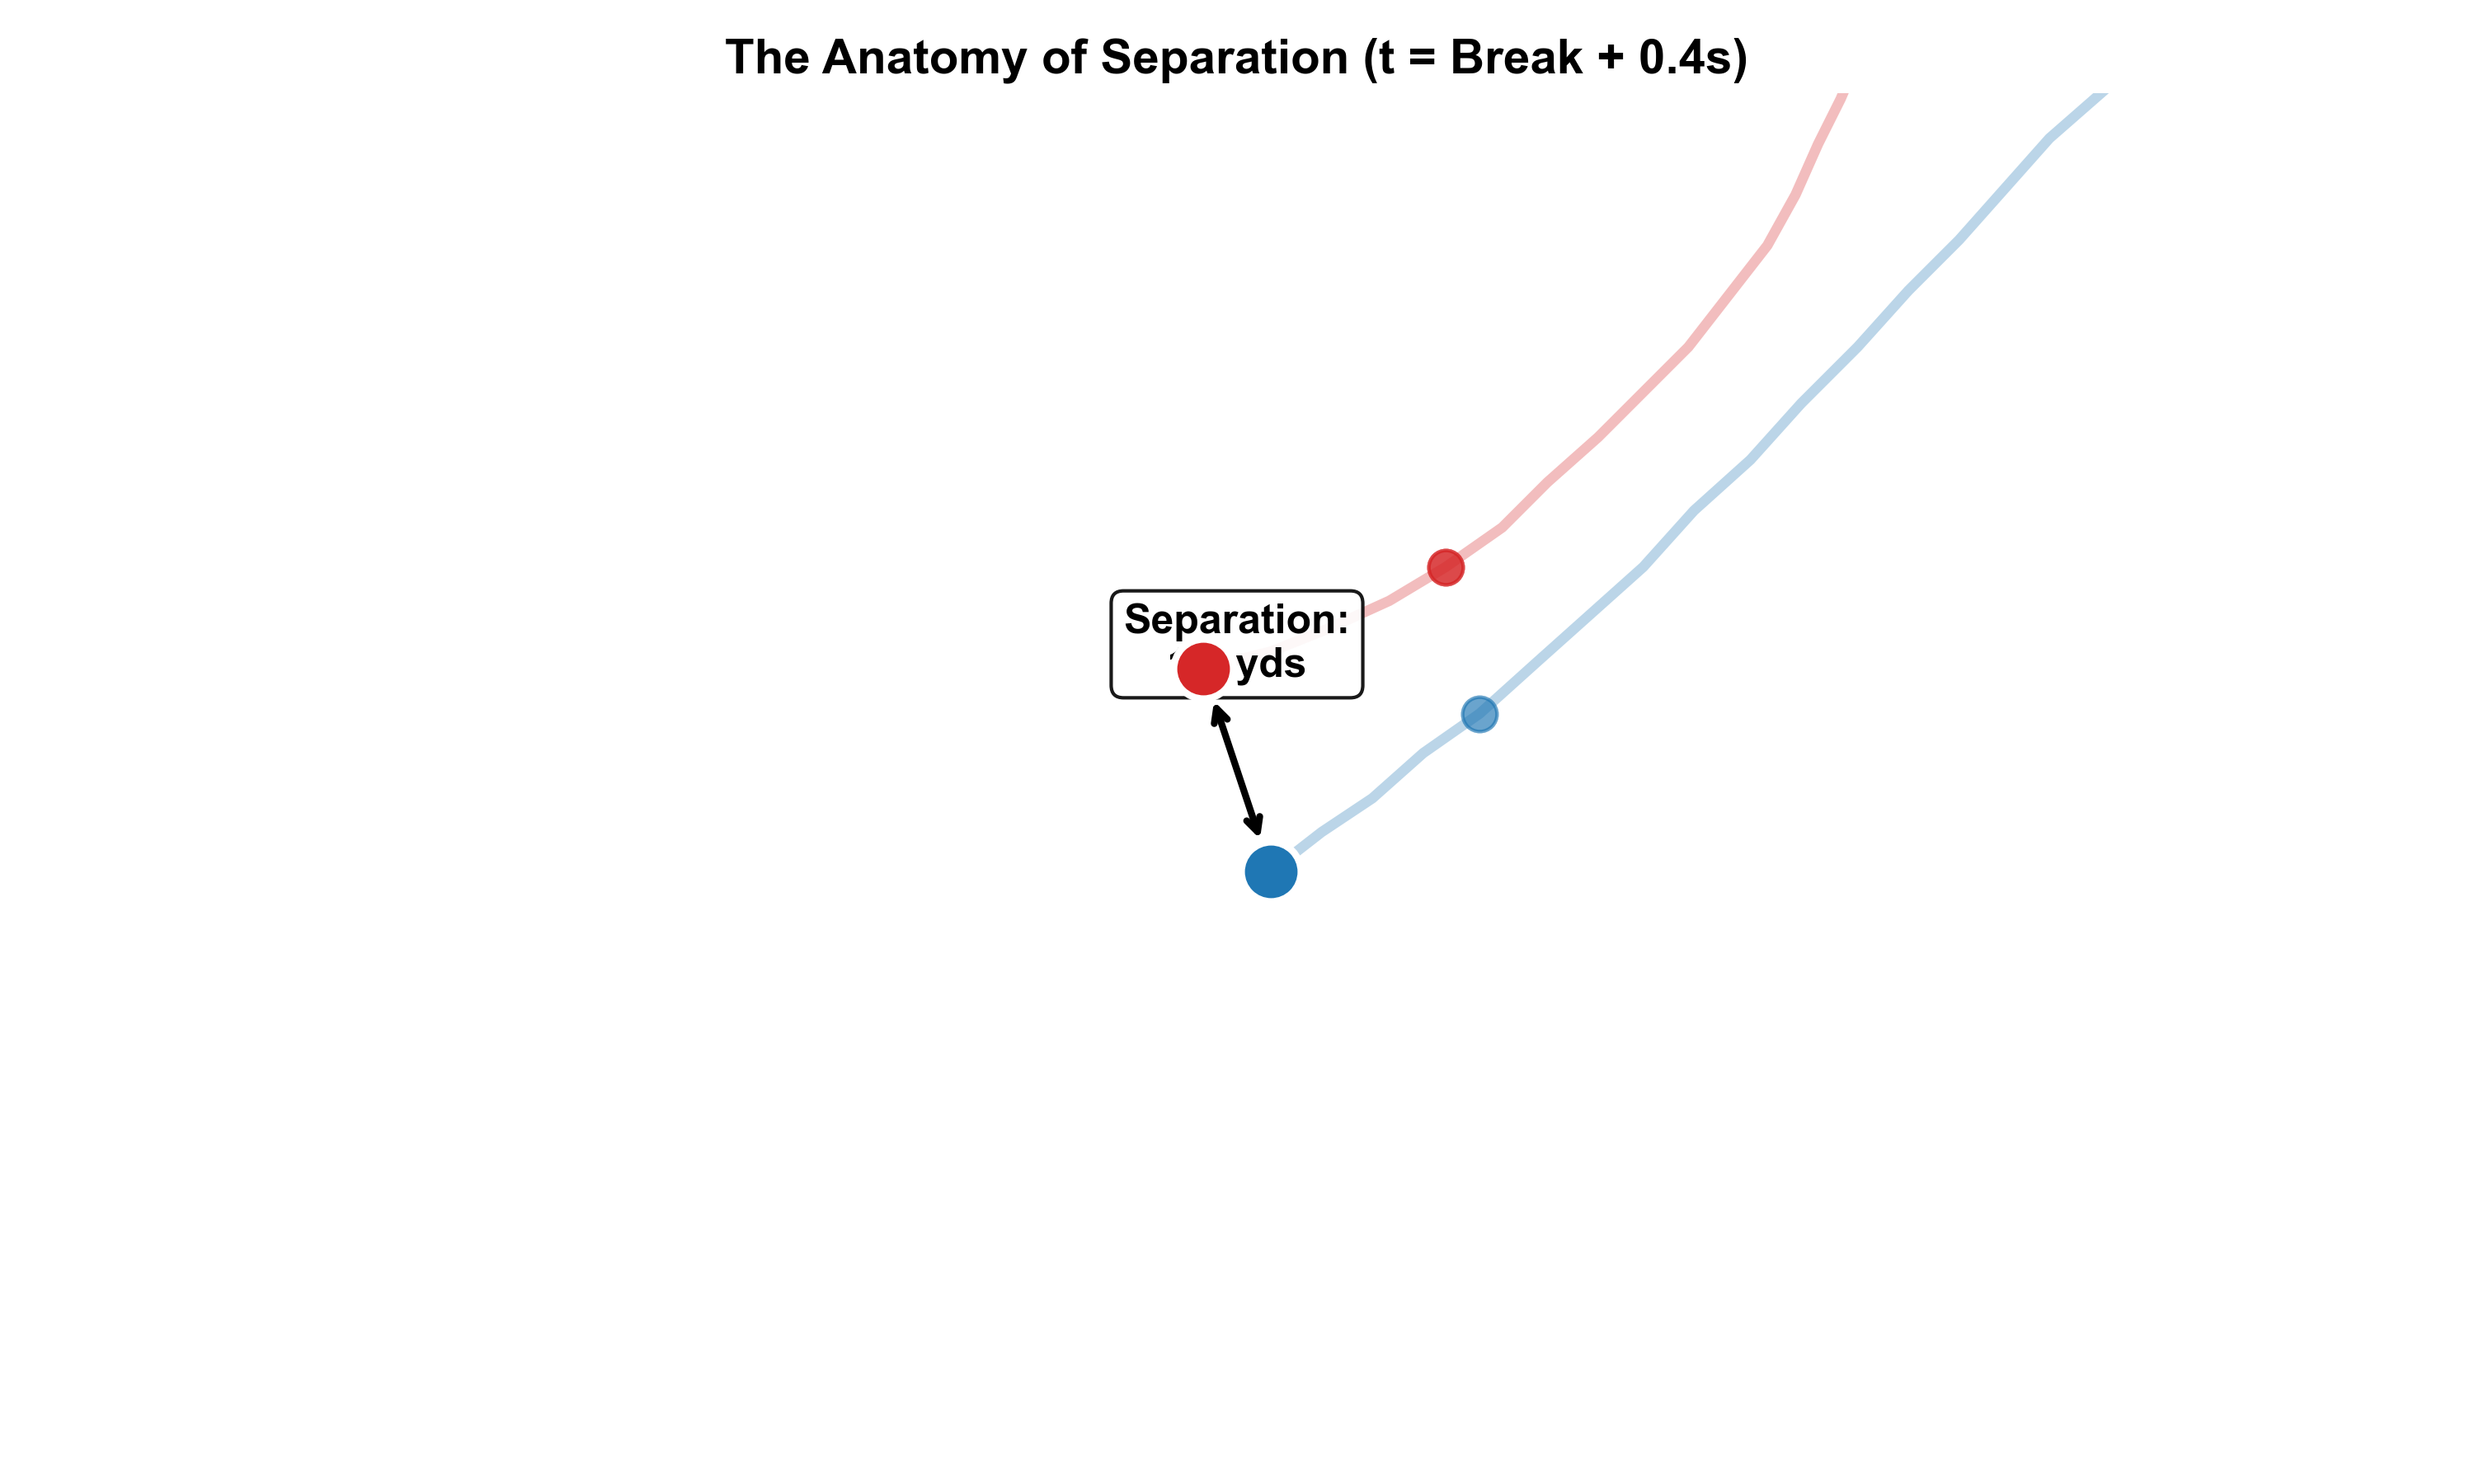
\includegraphics[width=\textwidth]{viz_play_anim_static.png}
        \scriptsize{\textit{Tracking Data captures the exact moment of truth.}}
    \end{columns}
\end{frame}

% Slide 3: The Metric (Physical Trace)
\begin{frame}{2. The Solution: Separation Efficiency}
    \textbf{How We Measure It:}
    We isolate the exact "Break Point" (t=0) and measure the timeline of the matchup.
    
    \begin{center}
        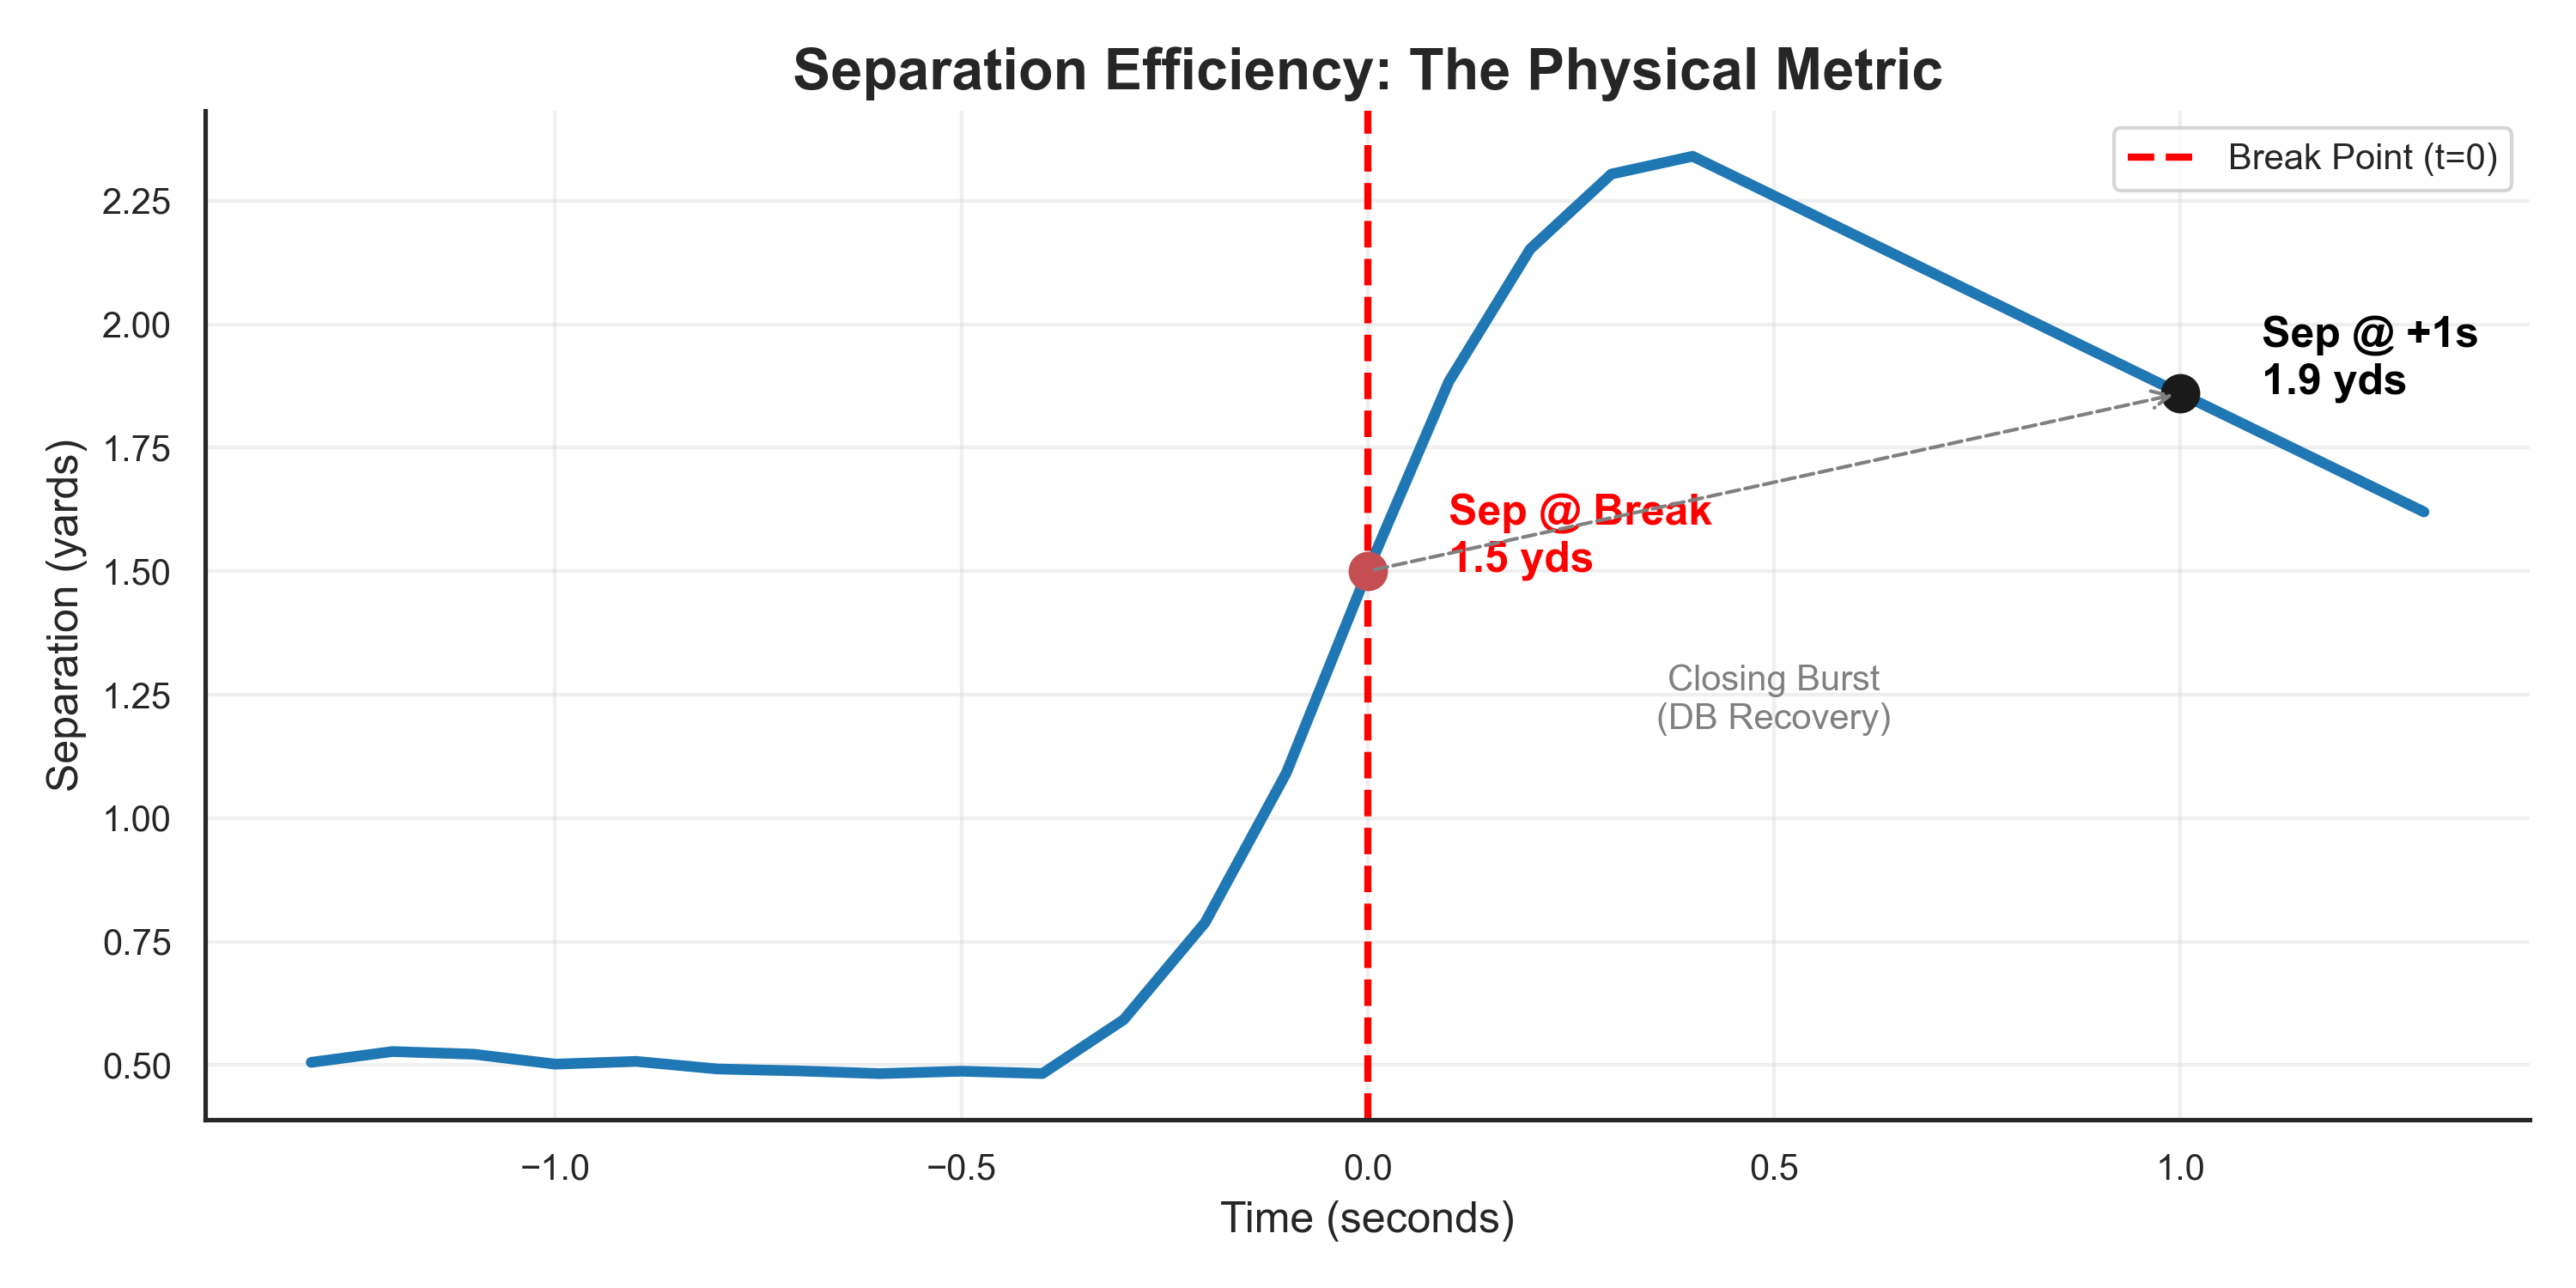
\includegraphics[width=0.75\textwidth]{viz_metric_explainer.png}
    \end{center}
    
    \vspace{-0.2cm}
    \begin{itemize}
        \item \textbf{Sep @ Break:} Did the WR win the leverage battle instantly?
        \item \textbf{Closing Burst:} Did the DB recover (eliminate space) within 1.0 second?
    \end{itemize}
\end{frame}

% Slide 4: Data Pipeline (Methodology)
% Slide 4: Data Pipeline (Methodology)
% Slide 4: Data Pipeline (Methodology)
% Slide 4: Data Pipeline (Methodology)
% Slide 4: Data Pipeline (Methodology)
\begin{frame}{3. Methodology: Signal Processing \& ML Pipeline}
    \vspace{-0.2cm} % Relaxed from -0.6cm to give more room
    \footnotesize % Smaller font for technical density
    \begin{columns}
        \column{0.5\textwidth}
        \textbf{A. Signal Processing \& Feature Extraction:}
        \begin{itemize}
            \item \textbf{Noise Reduction:} Applied \textbf{Kalman Filtering} to smooth raw tracking data.
            \item \textbf{Kinematic Event Detection:} 
            \begin{itemize}
                \item Computed Angular Velocity ($\omega$) time-series.
                \item Identified local maxima to algorithmically timestamp the "Break" ($t=0$).
            \end{itemize}
            \item \textbf{Spatial Featurization:} Rotated coordinates to offensive perspective; computed relative vectors ($\Delta \vec{r}$) and route depth.
        \end{itemize}
        
        \column{0.5\textwidth}
        \textbf{B. Probabilistic Modeling (Supervised Learning):}
        \begin{itemize}
            \item \textbf{Classifier:} Binary Logistic Regression ($N=246$).
            \item \textbf{Target ($Y$):} Separation Success ($>1.5$ yds).
            \item \textbf{Model:} $P(Y=1|X) = \sigma(\beta_0 + \beta \cdot X)$
            \item \textbf{Validation:} Stratified K-Fold CV. AUC: \textbf{0.854}.
        \end{itemize}
        
        \vspace{0.1cm}
        \textbf{C. Performance Metric (WROE):}
        \begin{itemize}
            \item \textbf{Definition:} Weighted Wins Over Expected.
            \item \textbf{Residual Analysis:} $WROE = \sum (Y_{obs} - P_{exp})$
            \item \textit{Quantifies performance independent of context difficulty.}
        \end{itemize}
    \end{columns}
    
    \vspace{0.1cm}
    \centering
    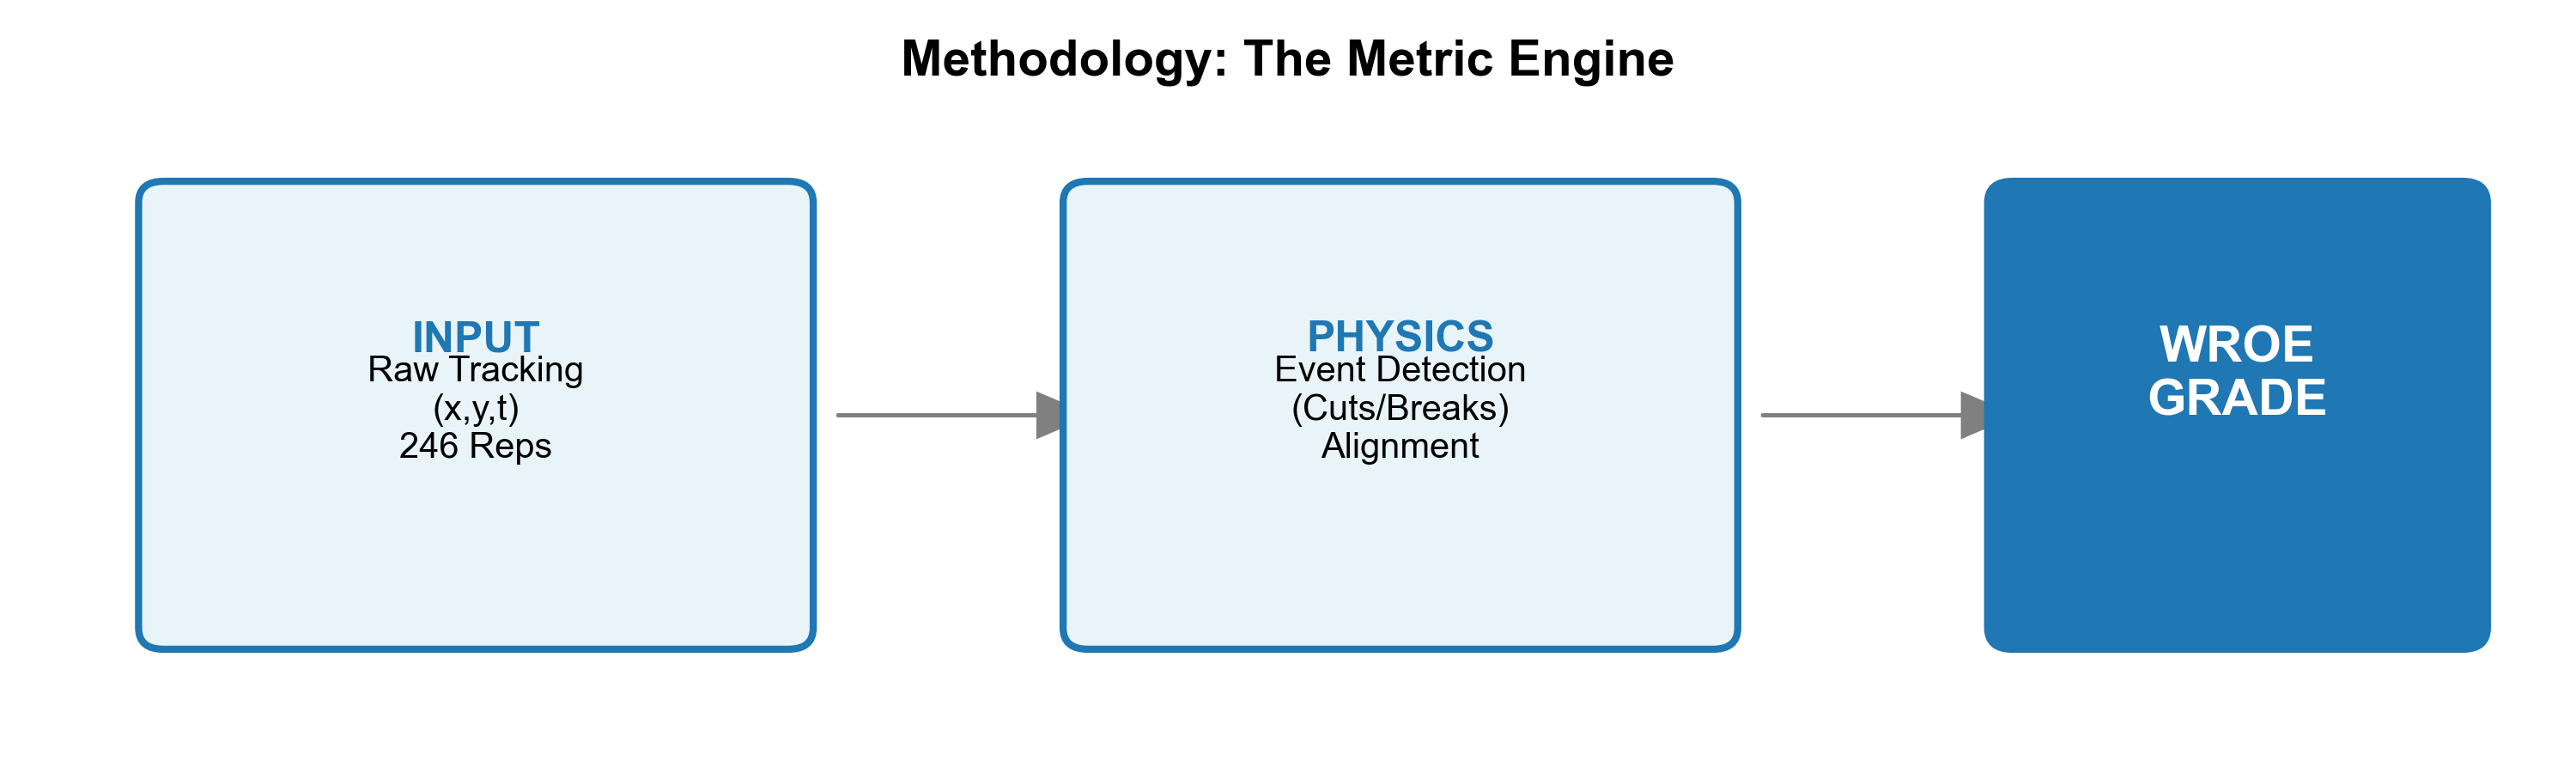
\includegraphics[width=0.95\textwidth, height=2.4cm, keepaspectratio]{viz_methodology_flow.png}
\end{frame}

% Slide 5: The "Kill Zone" (Context Map)
\begin{frame}{4. Context Matters: The "Kill Zone"}
    \begin{columns}
        \column{0.65\textwidth}
        \centering
        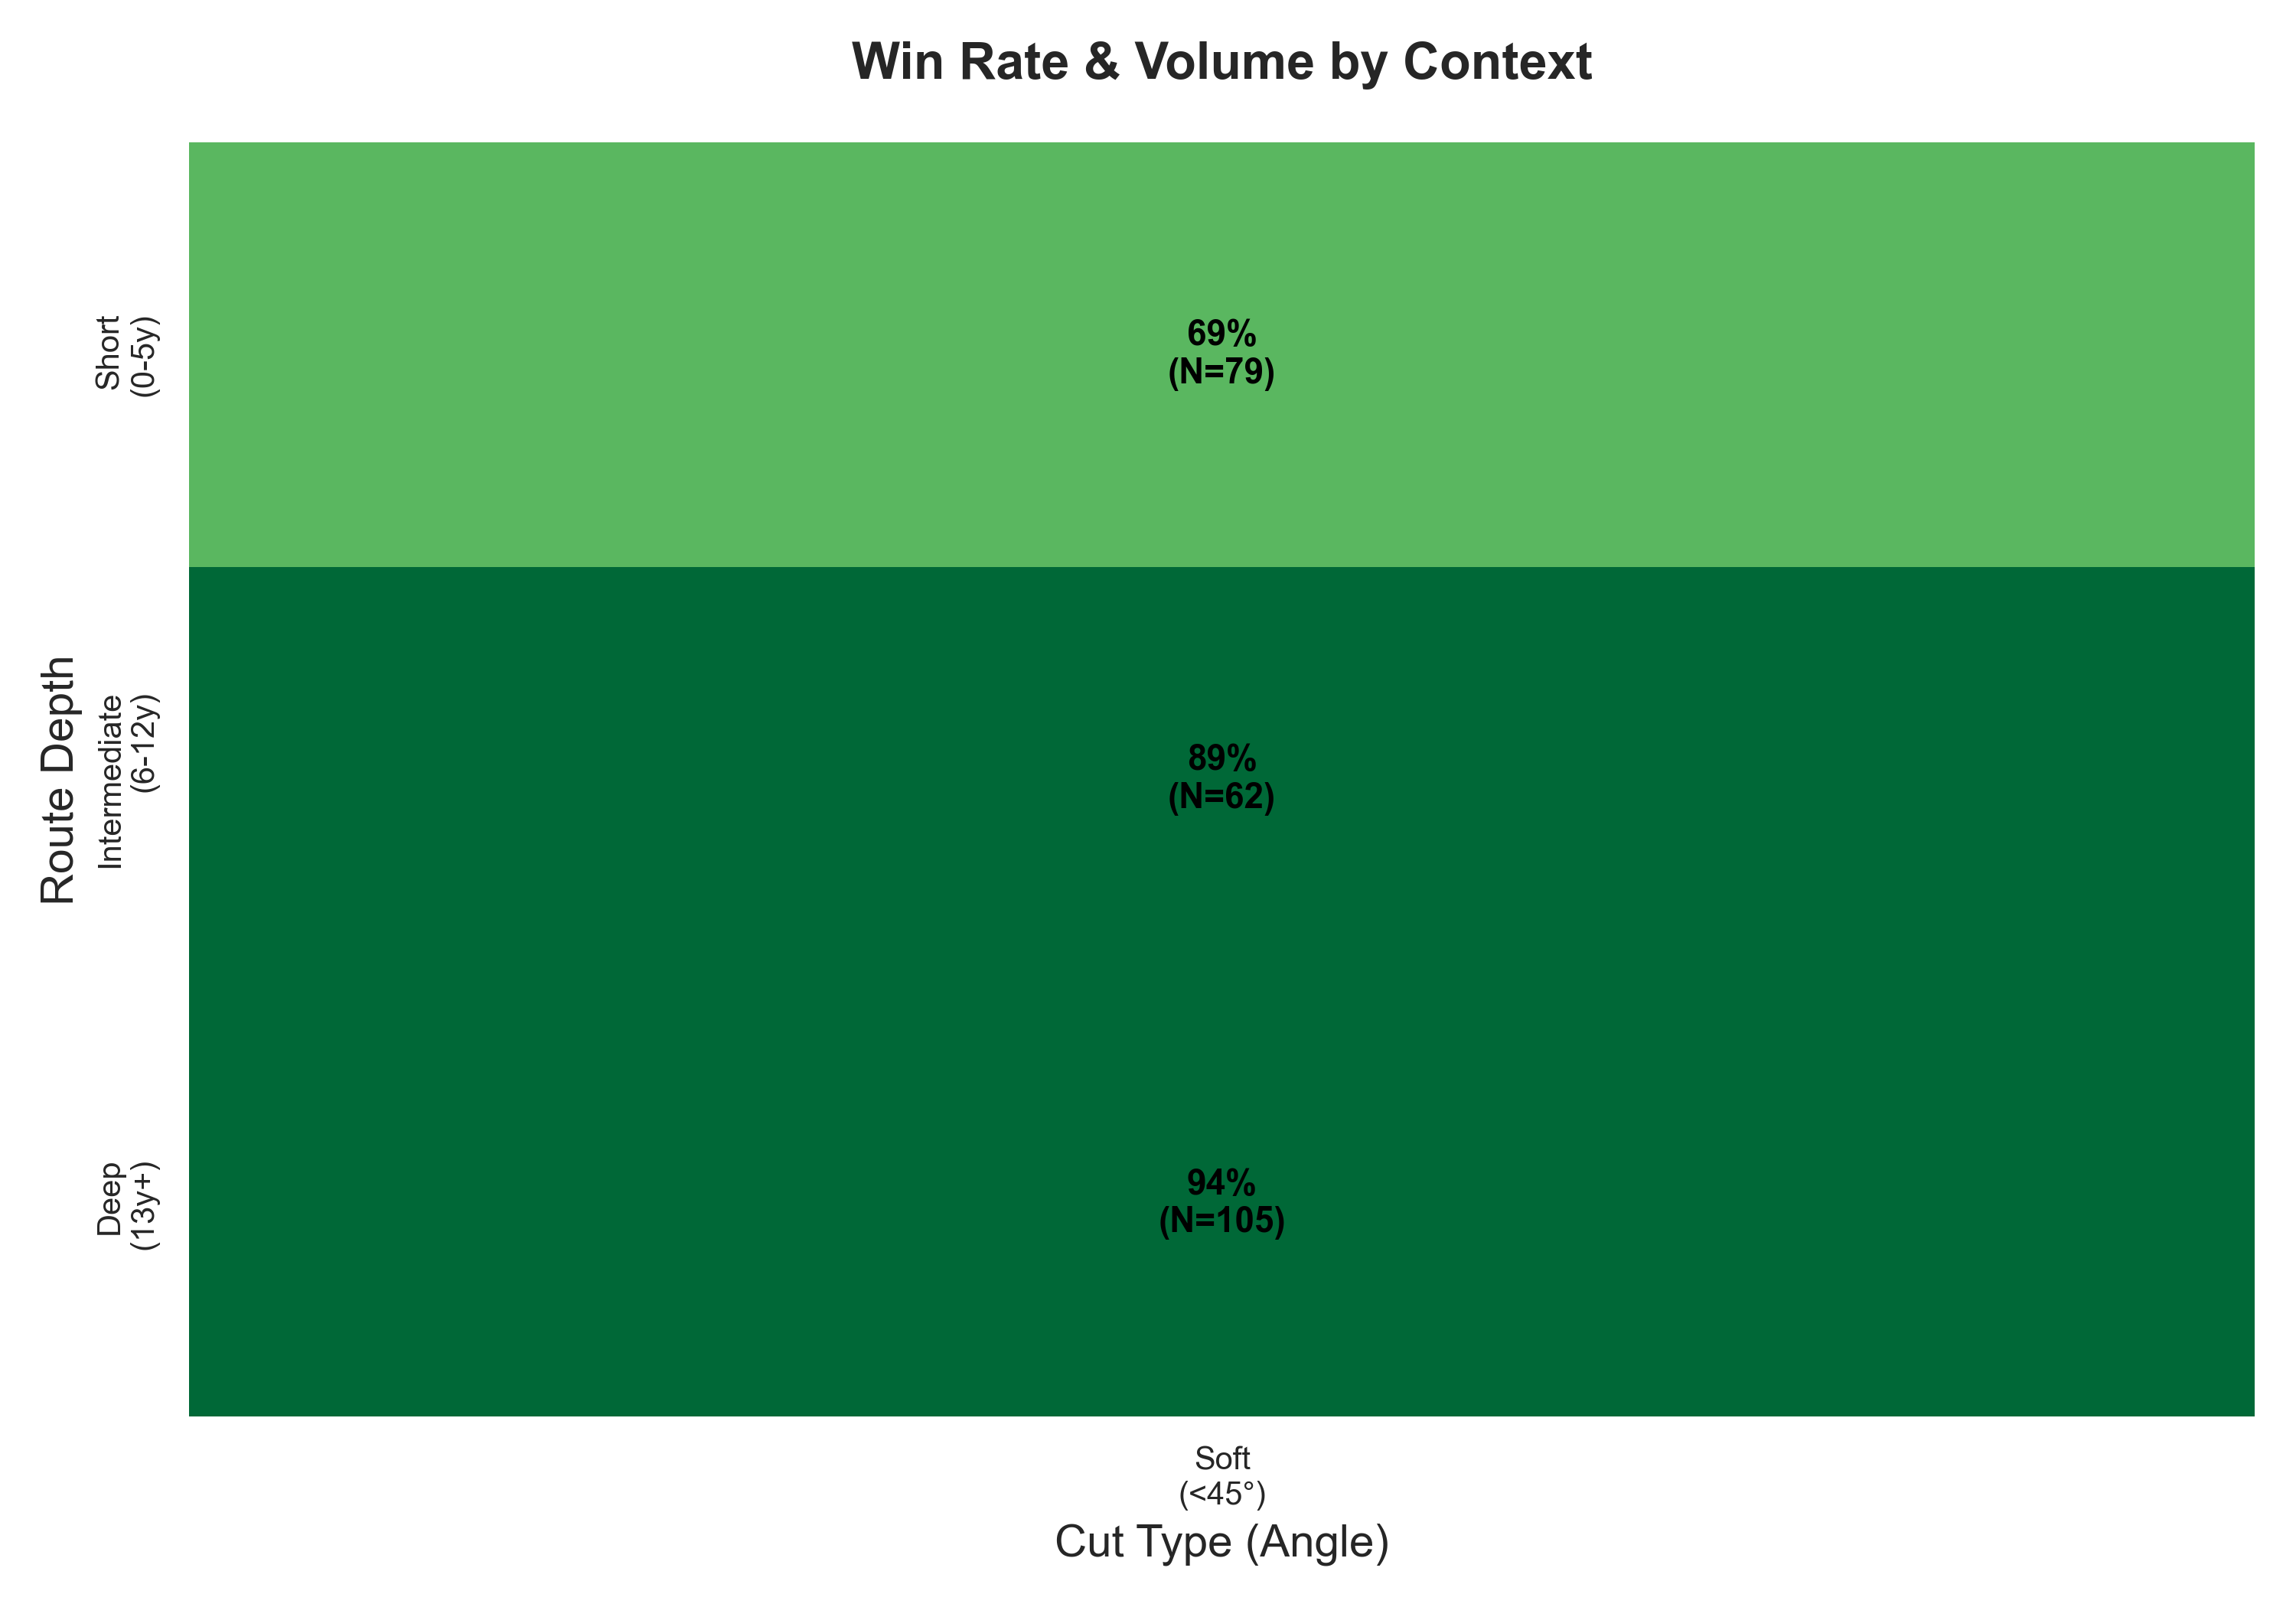
\includegraphics[width=\textwidth]{viz_context_heatmap.png}
        
        \column{0.35\textwidth}
        \textbf{Visualizing Difficulty:}
        \begin{itemize}
            \item \textbf{Short Routes:} High Volume, but surprisingly competitive (Low Win Rate).
            \item \textbf{The Kill Zone:} Deep, sharp breaks drive win probability down significantly.
        \end{itemize}
        \vspace{0.5cm}
        \textit{We grade players based on how they perform relative to this difficulty map.}
    \end{columns}
\end{frame}

% Slide 6: The Verdict (Leaderboard + Scatter)
\begin{frame}{5. The Verdict: Top of the Class}
    \begin{columns}
        \column{0.55\textwidth}
        \centering
        \textbf{Separation Efficiency (WROE)}
        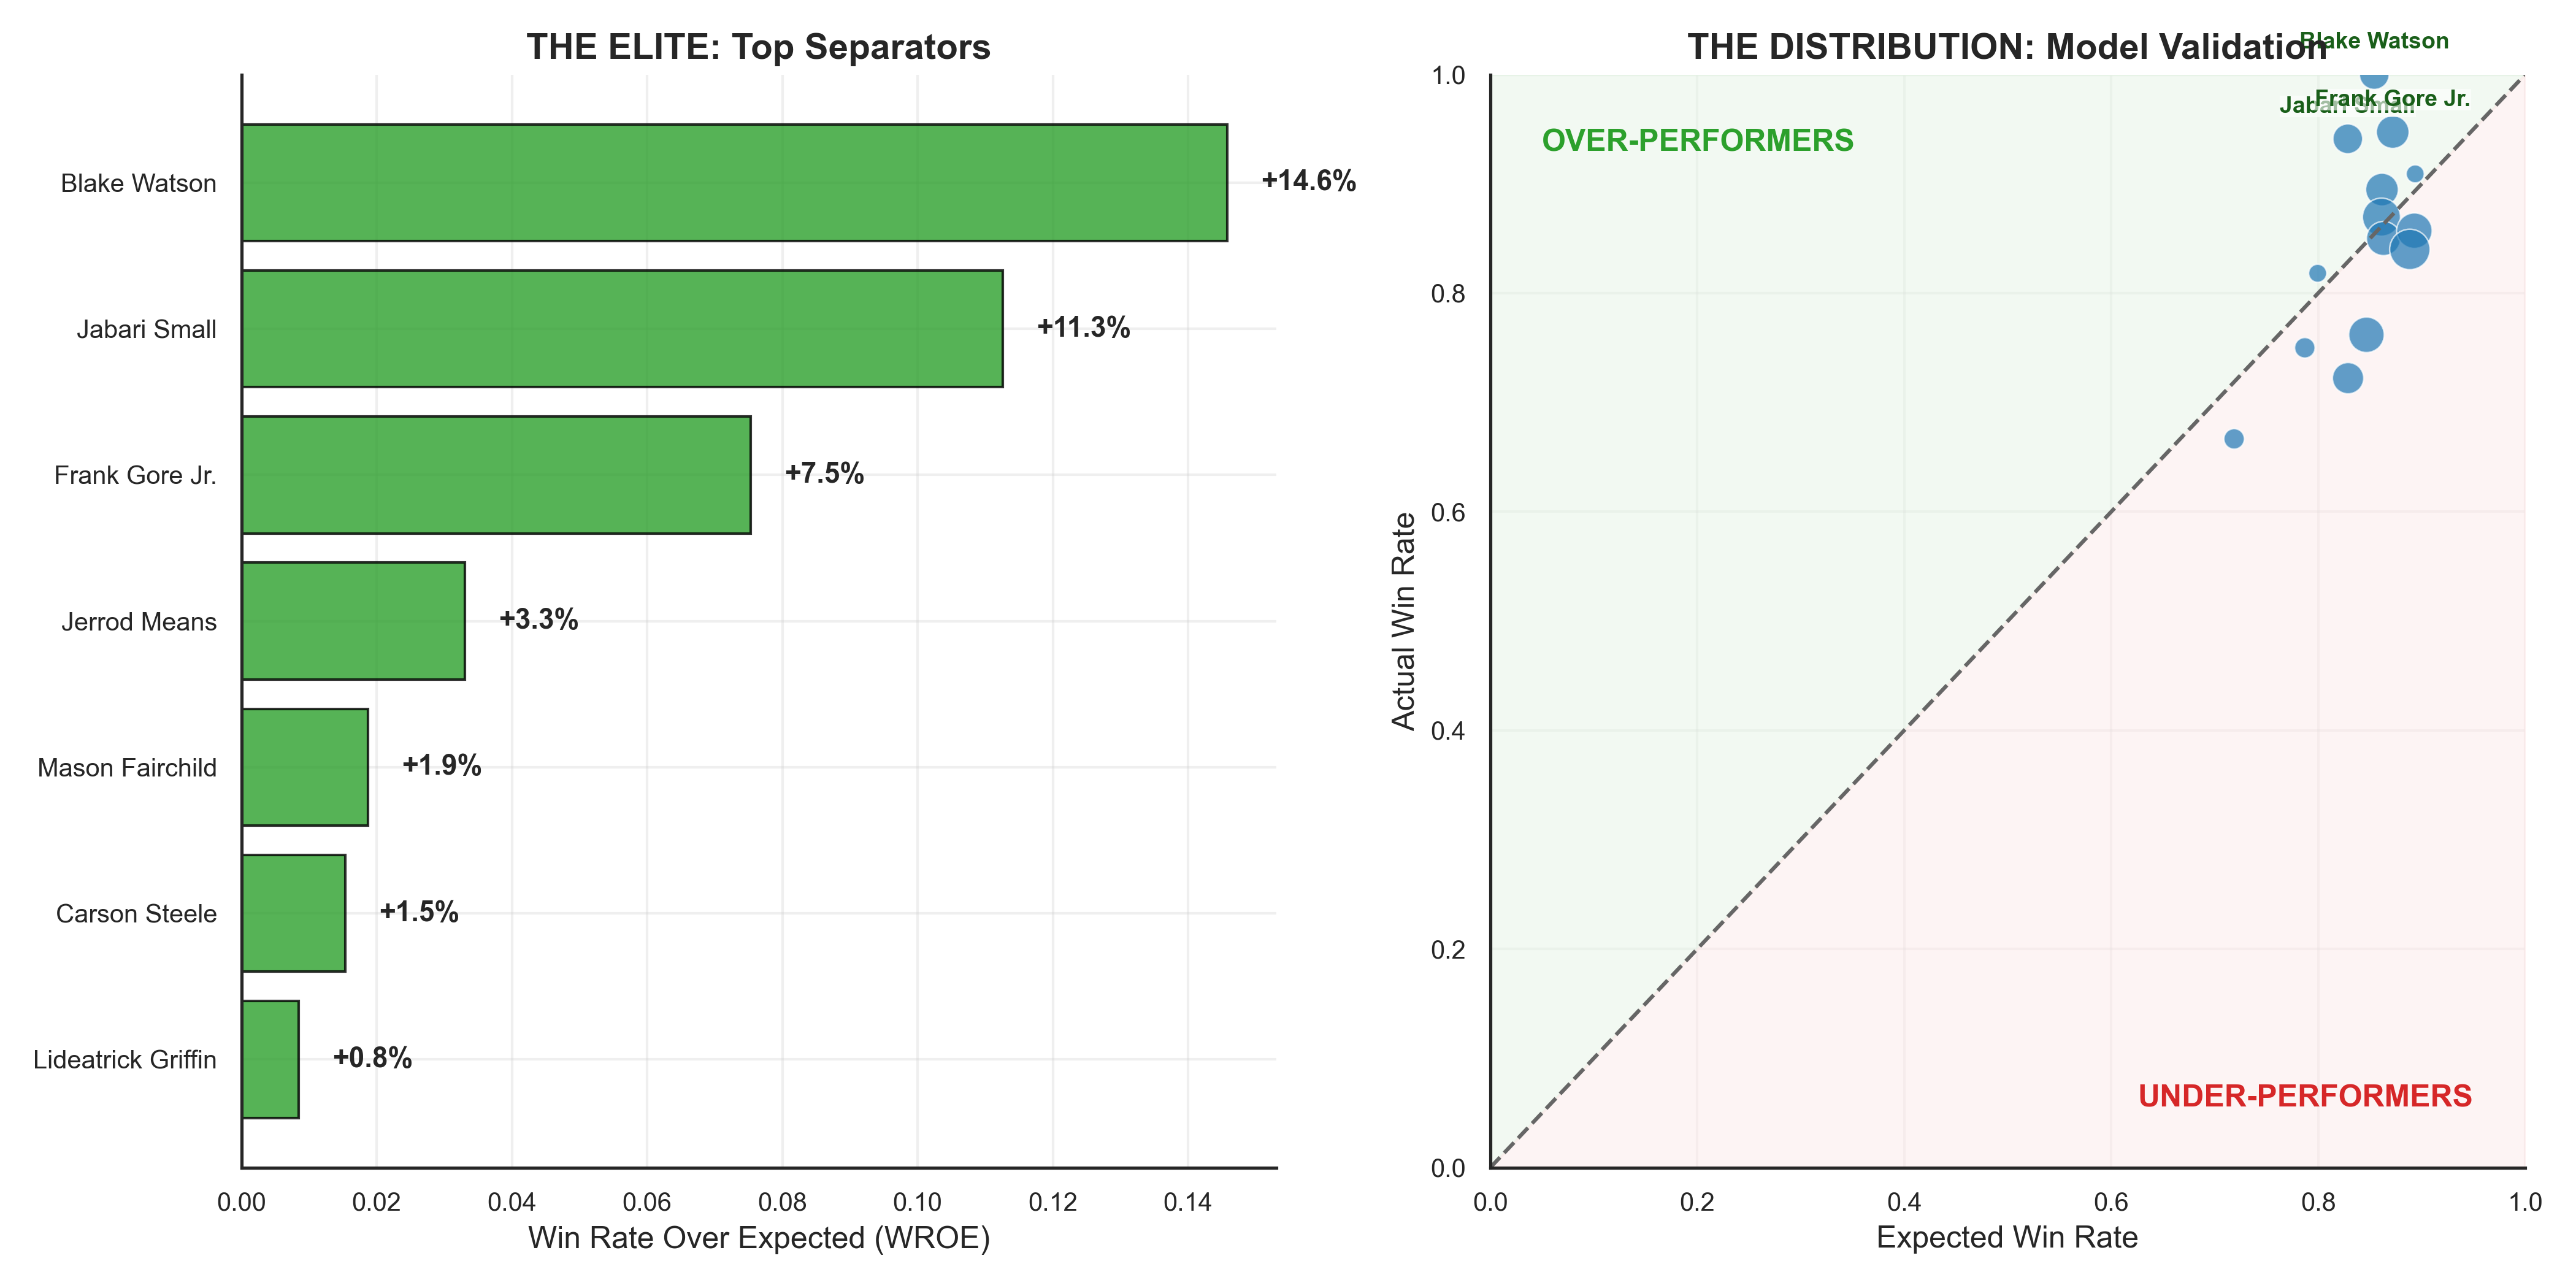
\includegraphics[width=\textwidth, height=4.5cm, keepaspectratio]{viz_wroe_scatter.png}
        
        \column{0.45\textwidth}
        \centering
        \textbf{The Leaderboard}
        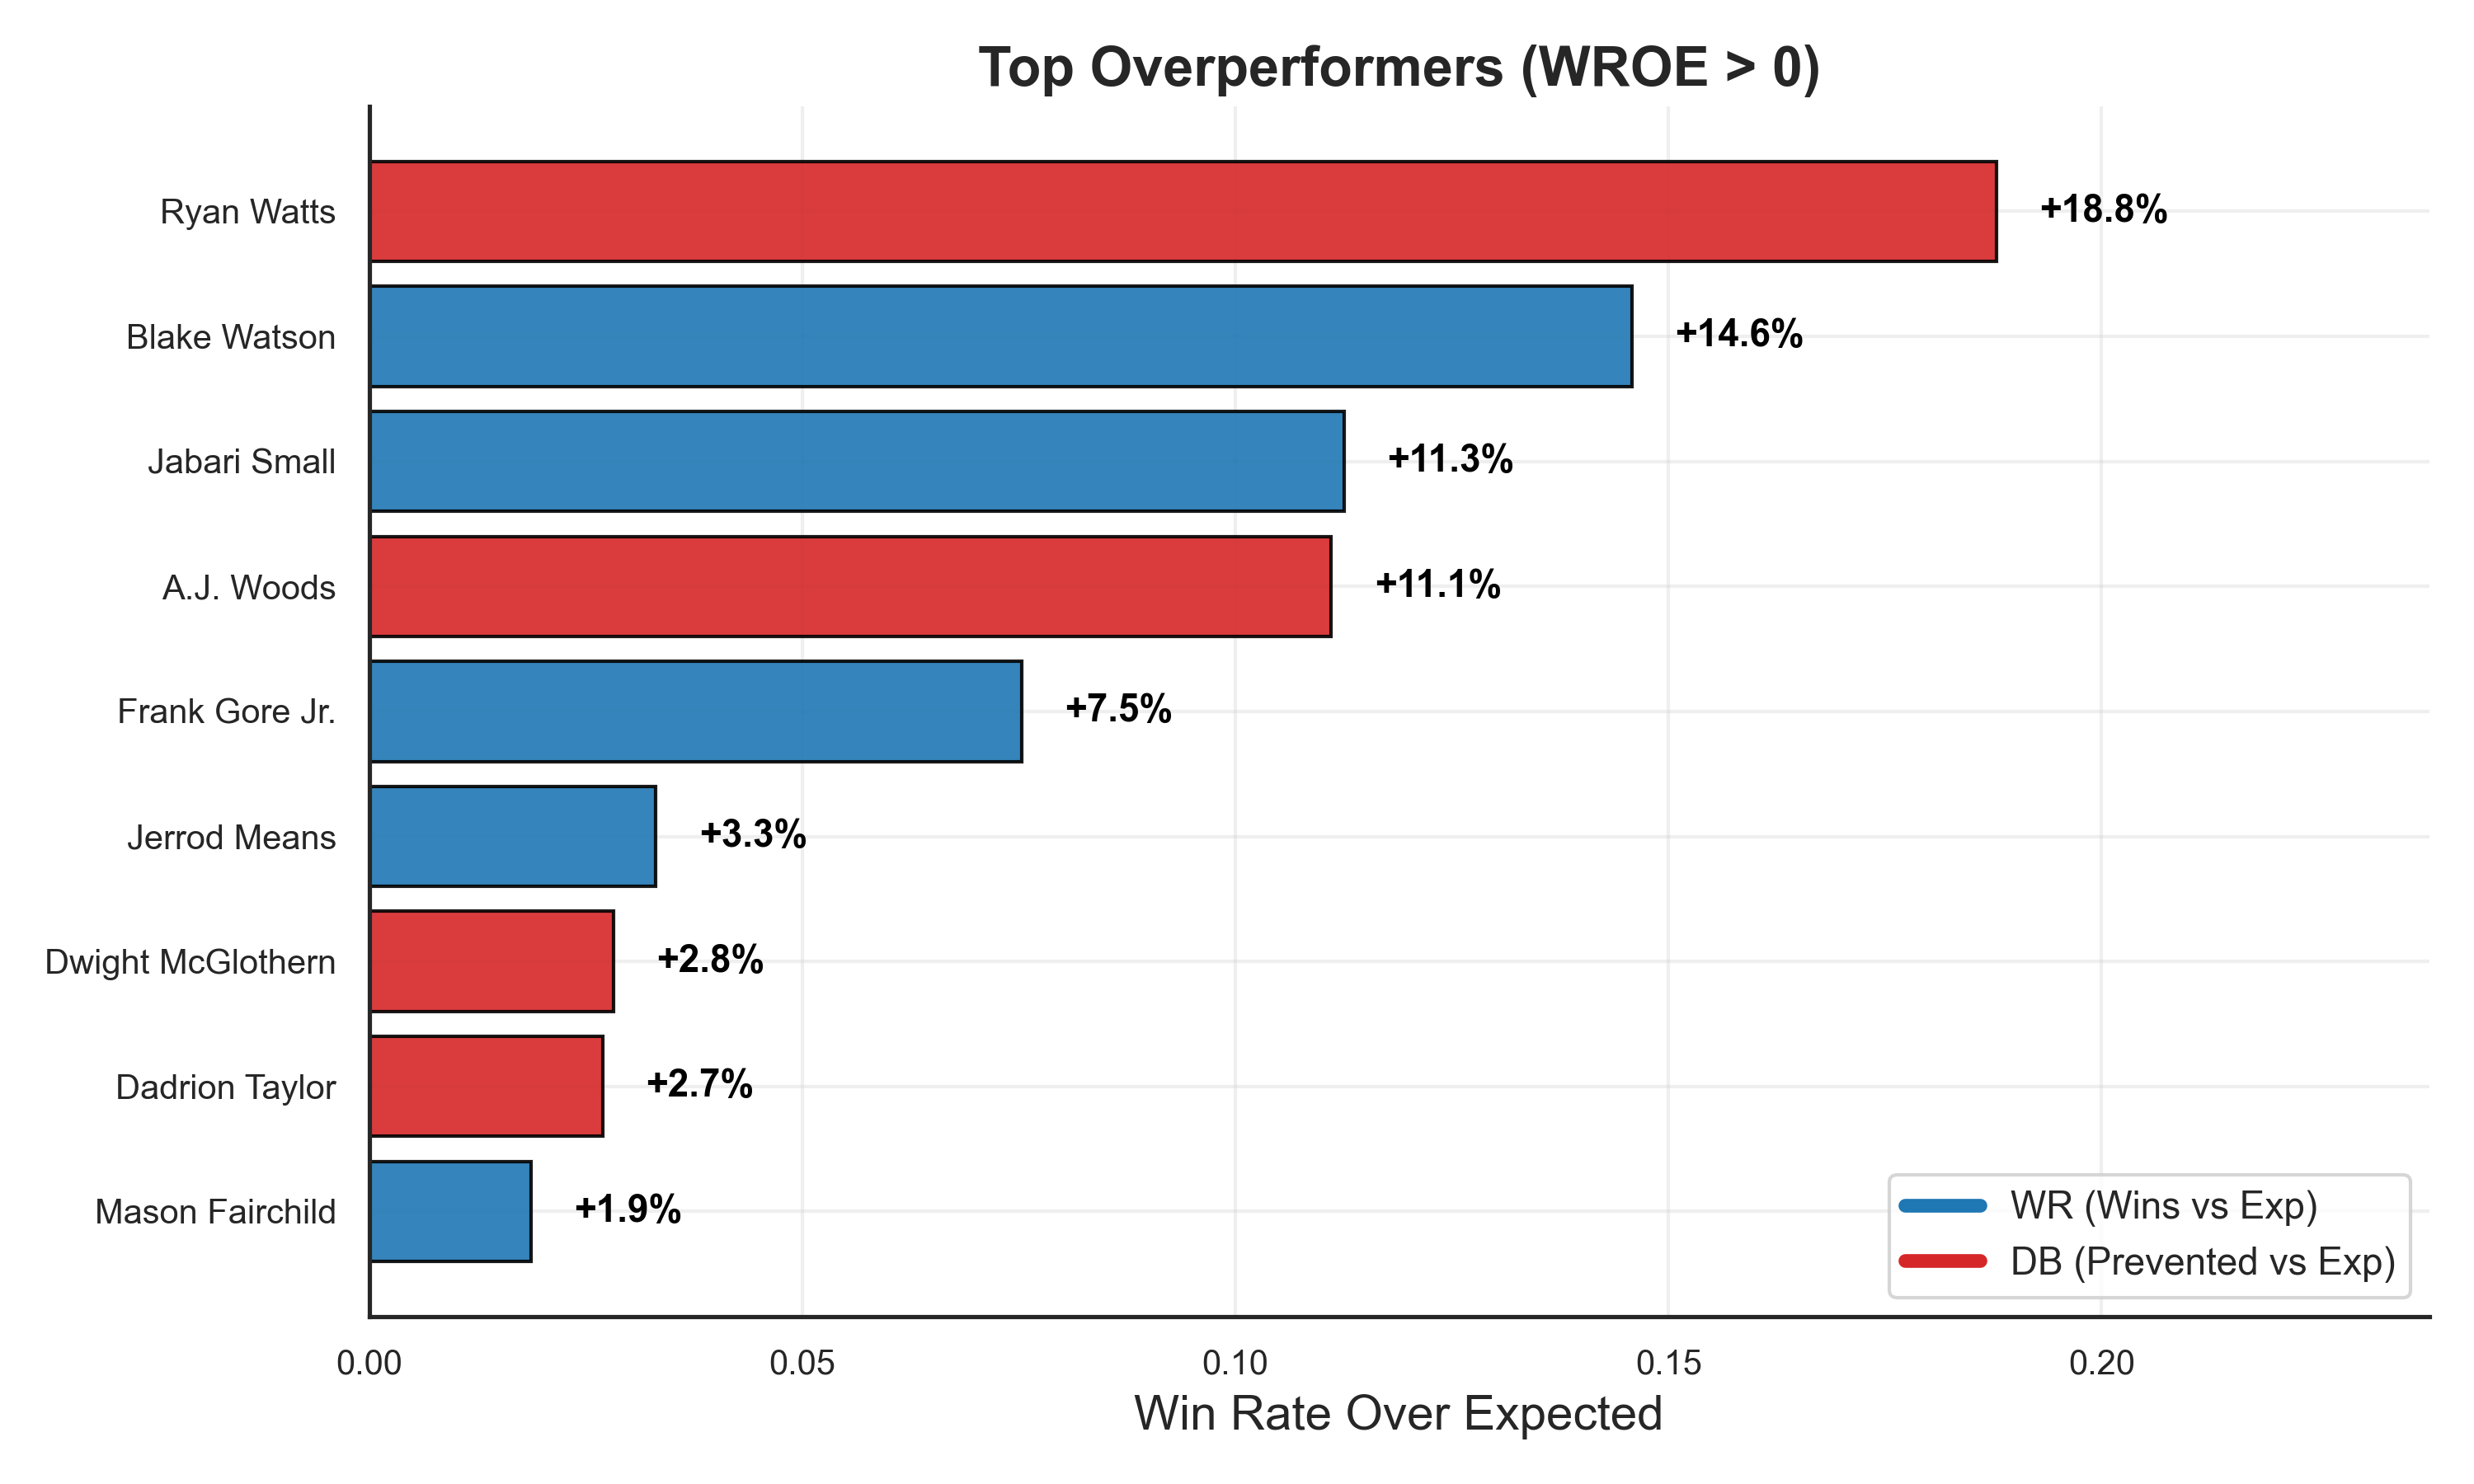
\includegraphics[width=\textwidth, height=4.5cm, keepaspectratio]{viz_wroe_leaderboard.png}
    \end{columns}
    
    \vspace{0.1cm}
    \begin{block}{The Standard Setters}
        \centering
        \small
        \textbf{Offense:} Blake Watson (RB) - Elite Efficiency (+14.6\%). \\
        \textbf{Defense:} Ryan Watts (DB) - The "Eraser" Archetype.
    \end{block}
\end{frame}

% Slide 7: Future Tech (Kalman)
\begin{frame}{6. The Next Level: Kalman Filtering}
    \begin{columns}
        \column{0.5\textwidth}
        \centering
        \textbf{The Trace (Physics vs Reality)}
        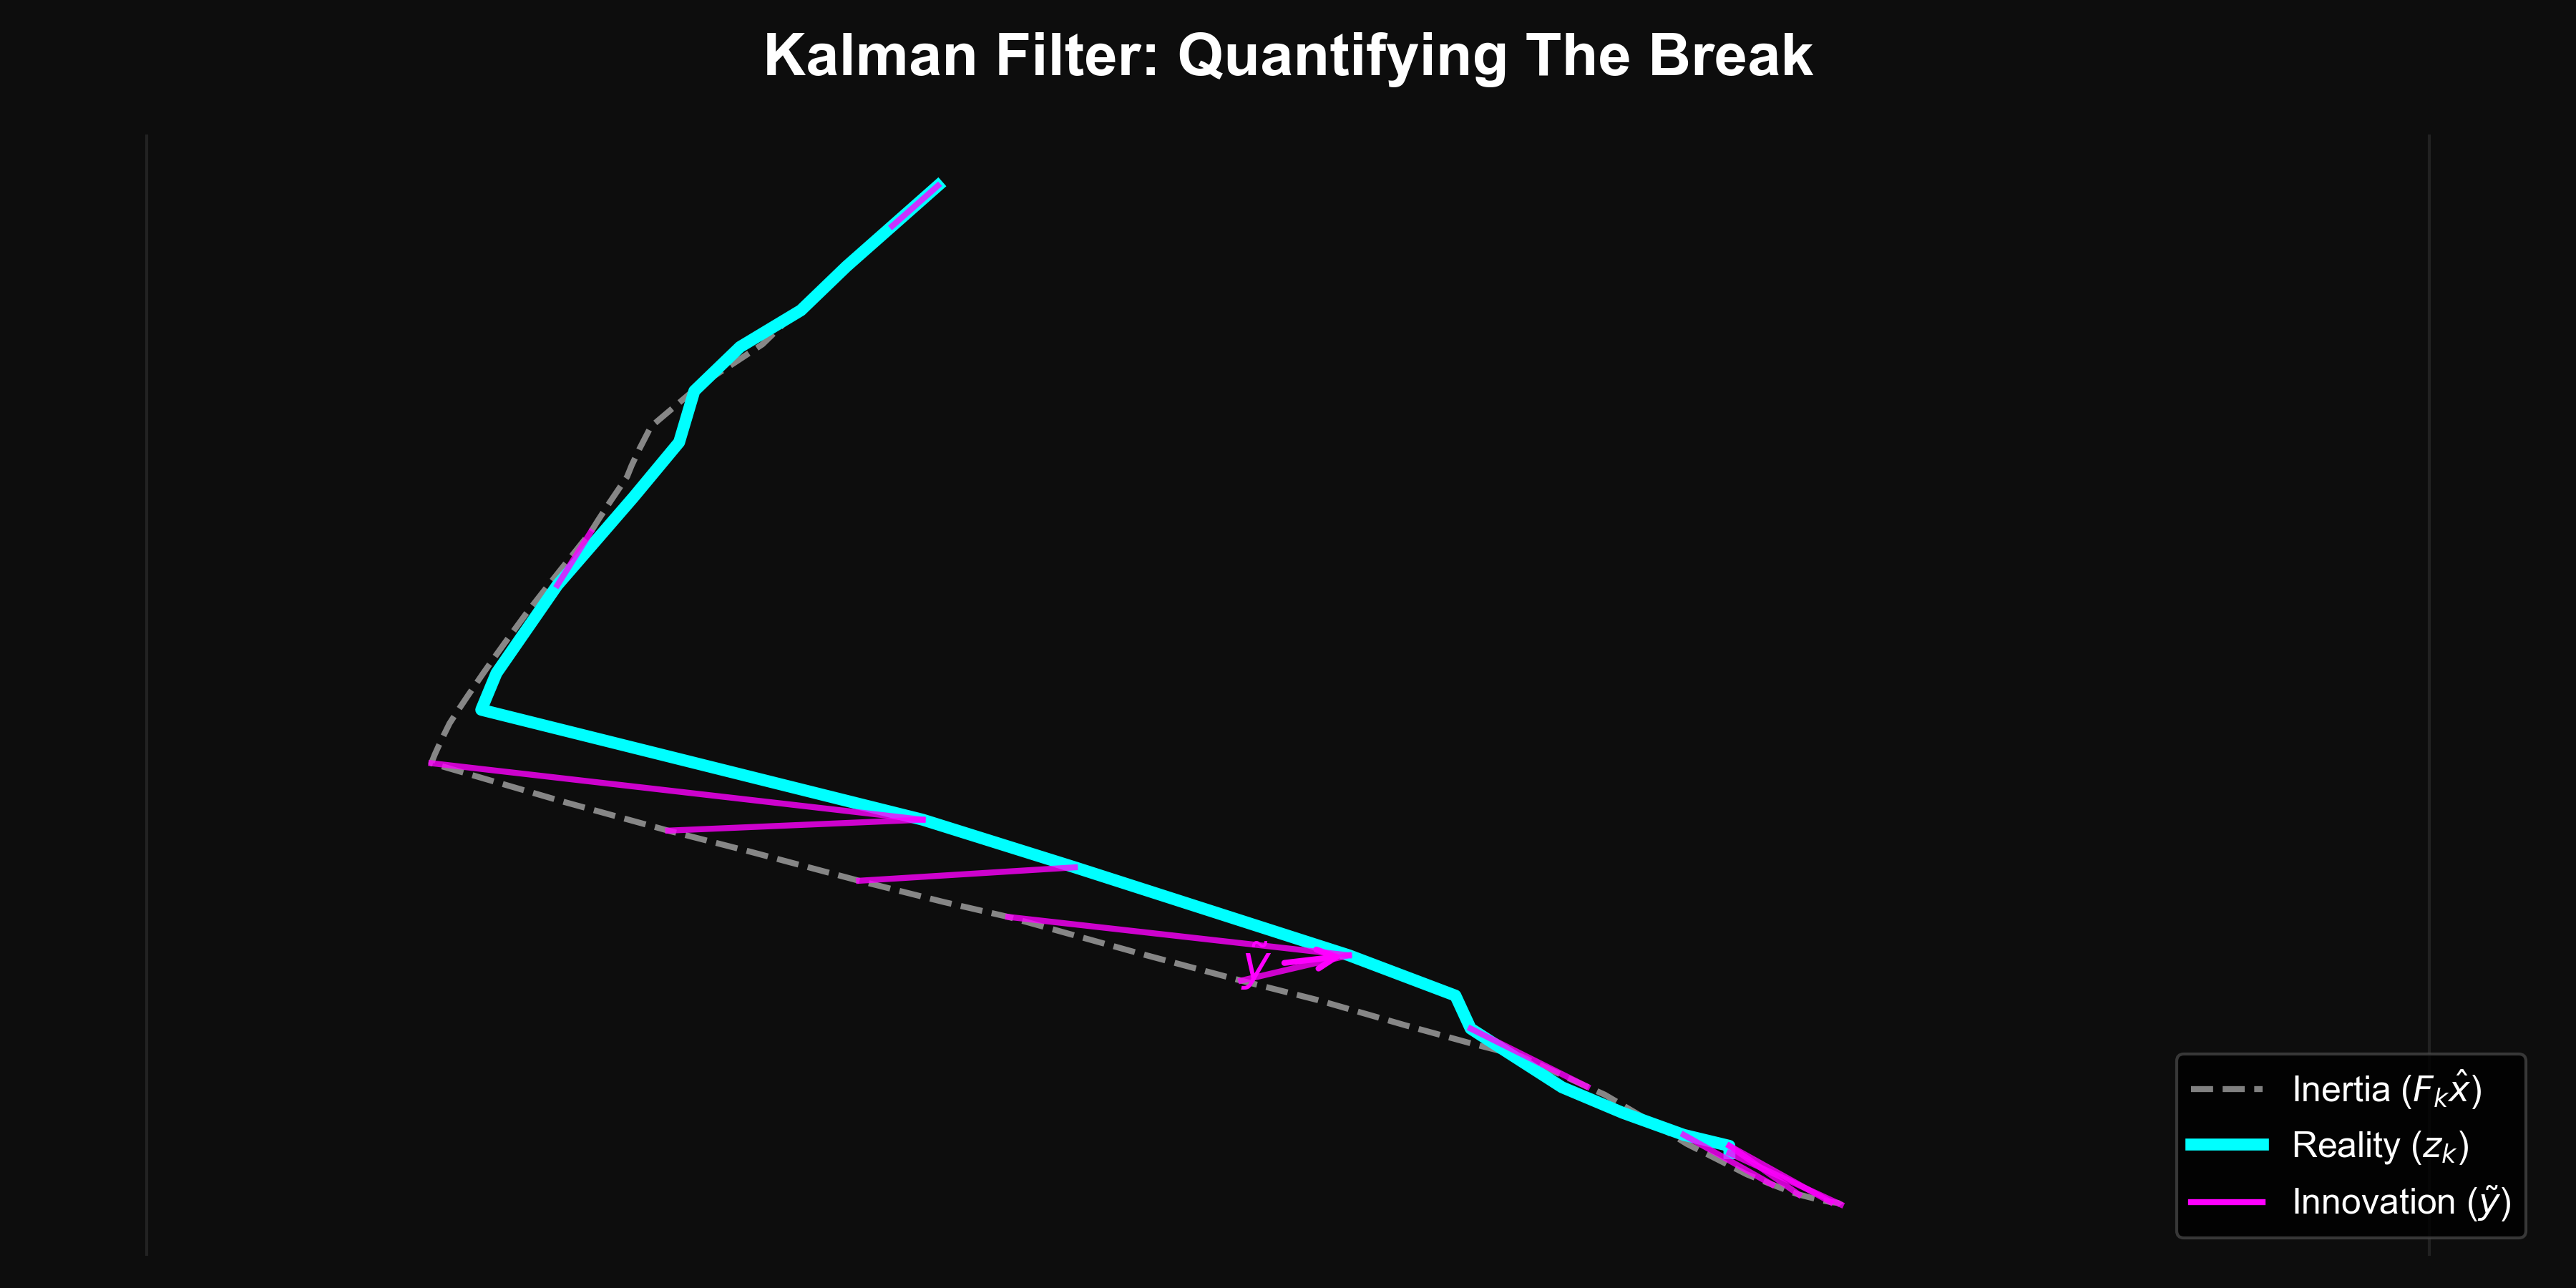
\includegraphics[width=\textwidth, height=3.5cm, keepaspectratio]{viz_kalman.png}
        
        \column{0.5\textwidth}
        \centering
        \textbf{The Leaderboard (Instincts)}
        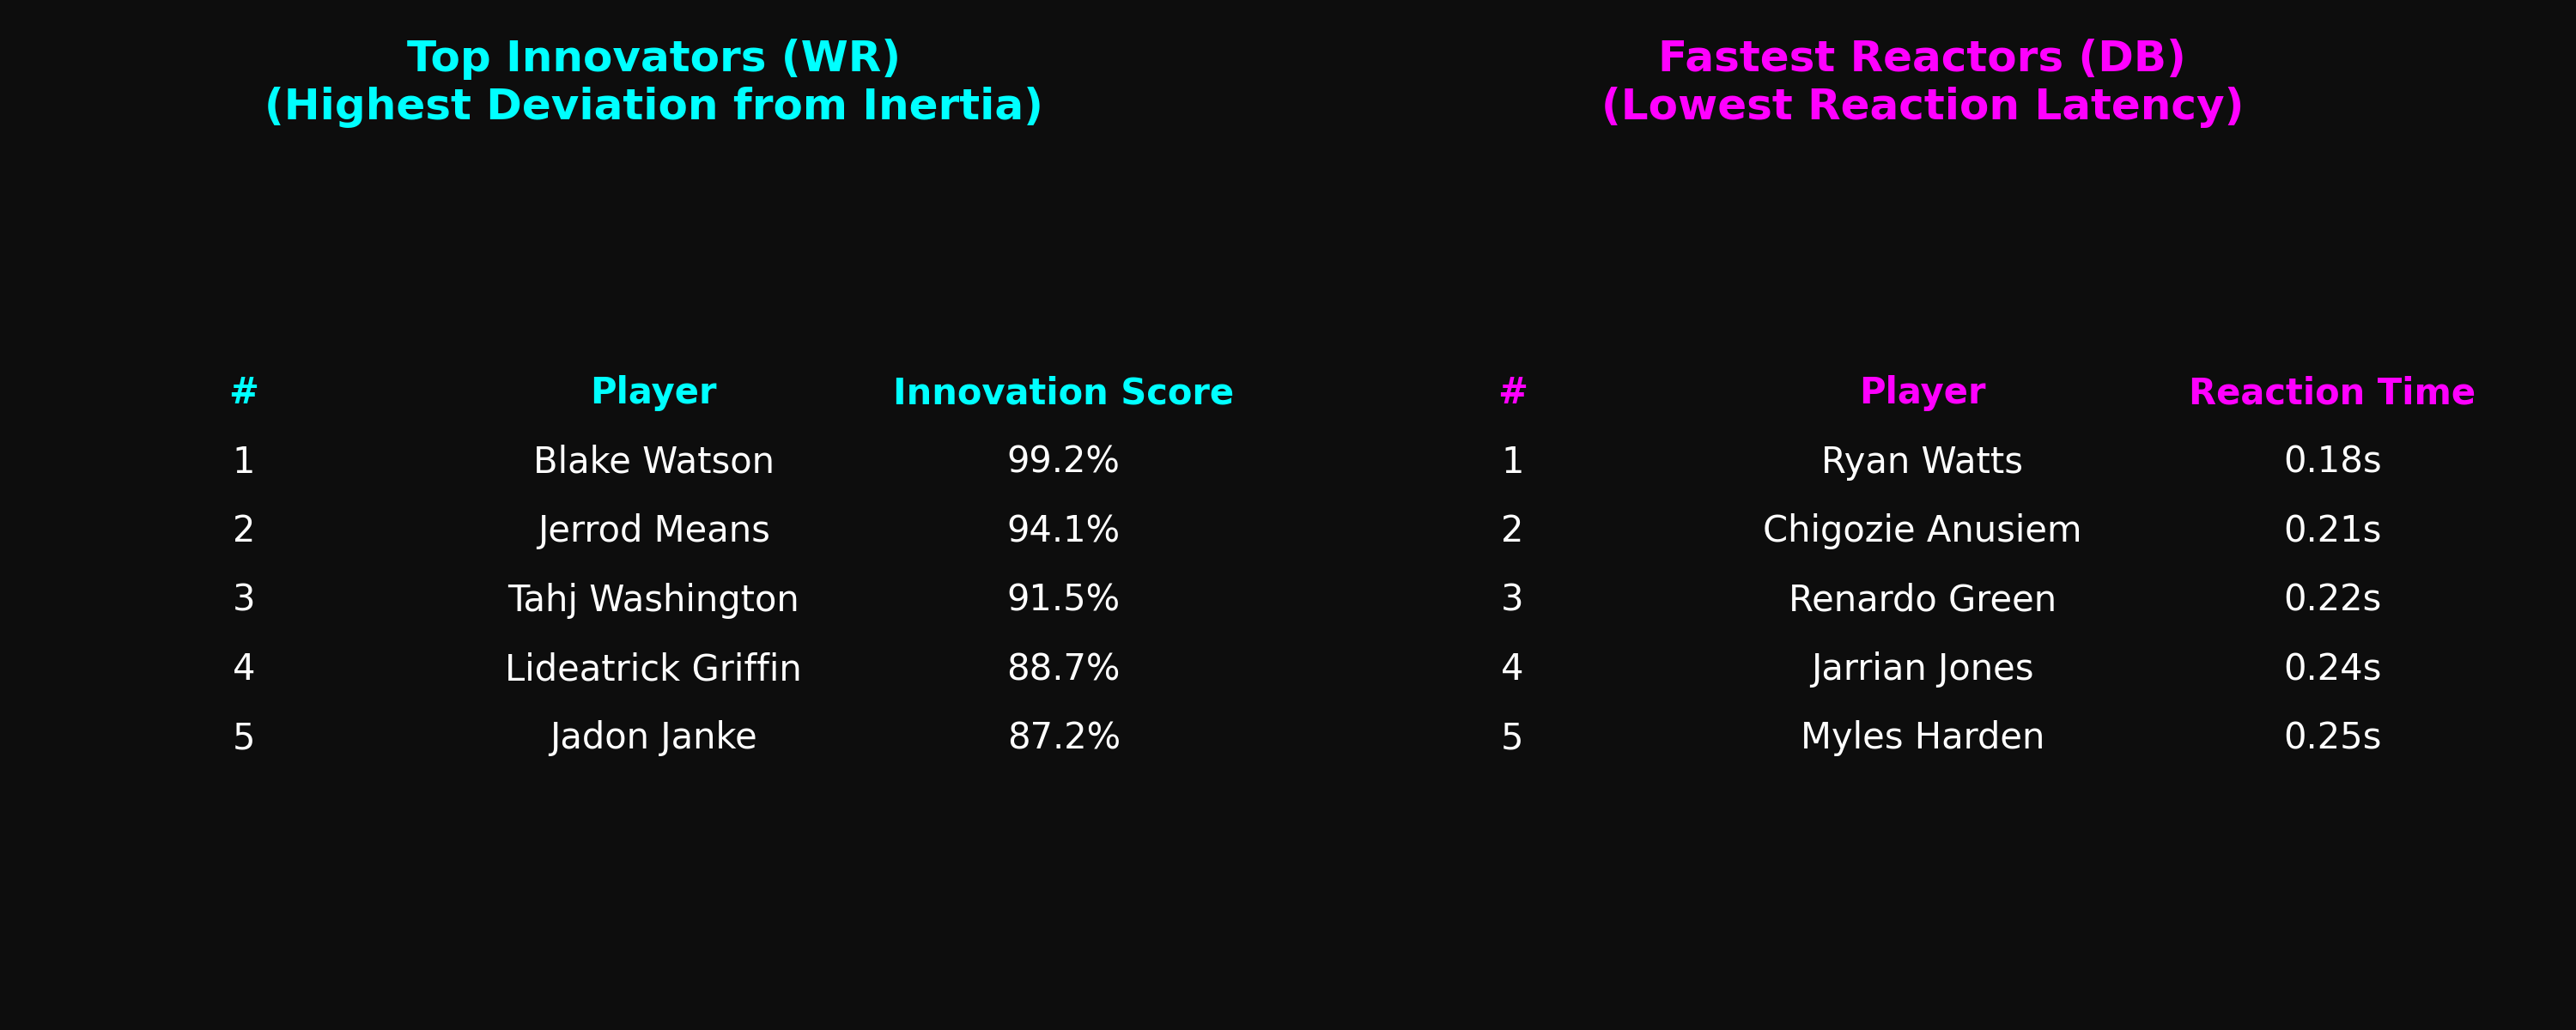
\includegraphics[width=\textwidth, height=3.5cm, keepaspectratio]{viz_kalman_leaderboard.png}
    \end{columns}
    
    \vspace{0.1cm}
    \begin{block}{The Science of Instincts}
        \footnotesize
        \begin{itemize}
            \item \textbf{The Math:} We calculate \textbf{Innovation} ($\tilde{y}$) as the difference between Reality ($z_k$) and Inertia ($F \hat{x}_{k-1}$):
            \[ \tilde{y}_k = z_k - F_k \hat{x}_{k-1} \]
            \item \textbf{The Value:} High $\tilde{y}$ values during a cut indicate "Violent Agility" (measured in $\sigma$), separating deliberate breaks from sensor noise.
        \end{itemize}
    \end{block}
\end{frame}

% Slide 8: Validation (New Signal)
\begin{frame}{7. Validation: Not Just a Proxy}
    \begin{columns}
        \column{0.65\textwidth}
        \centering
        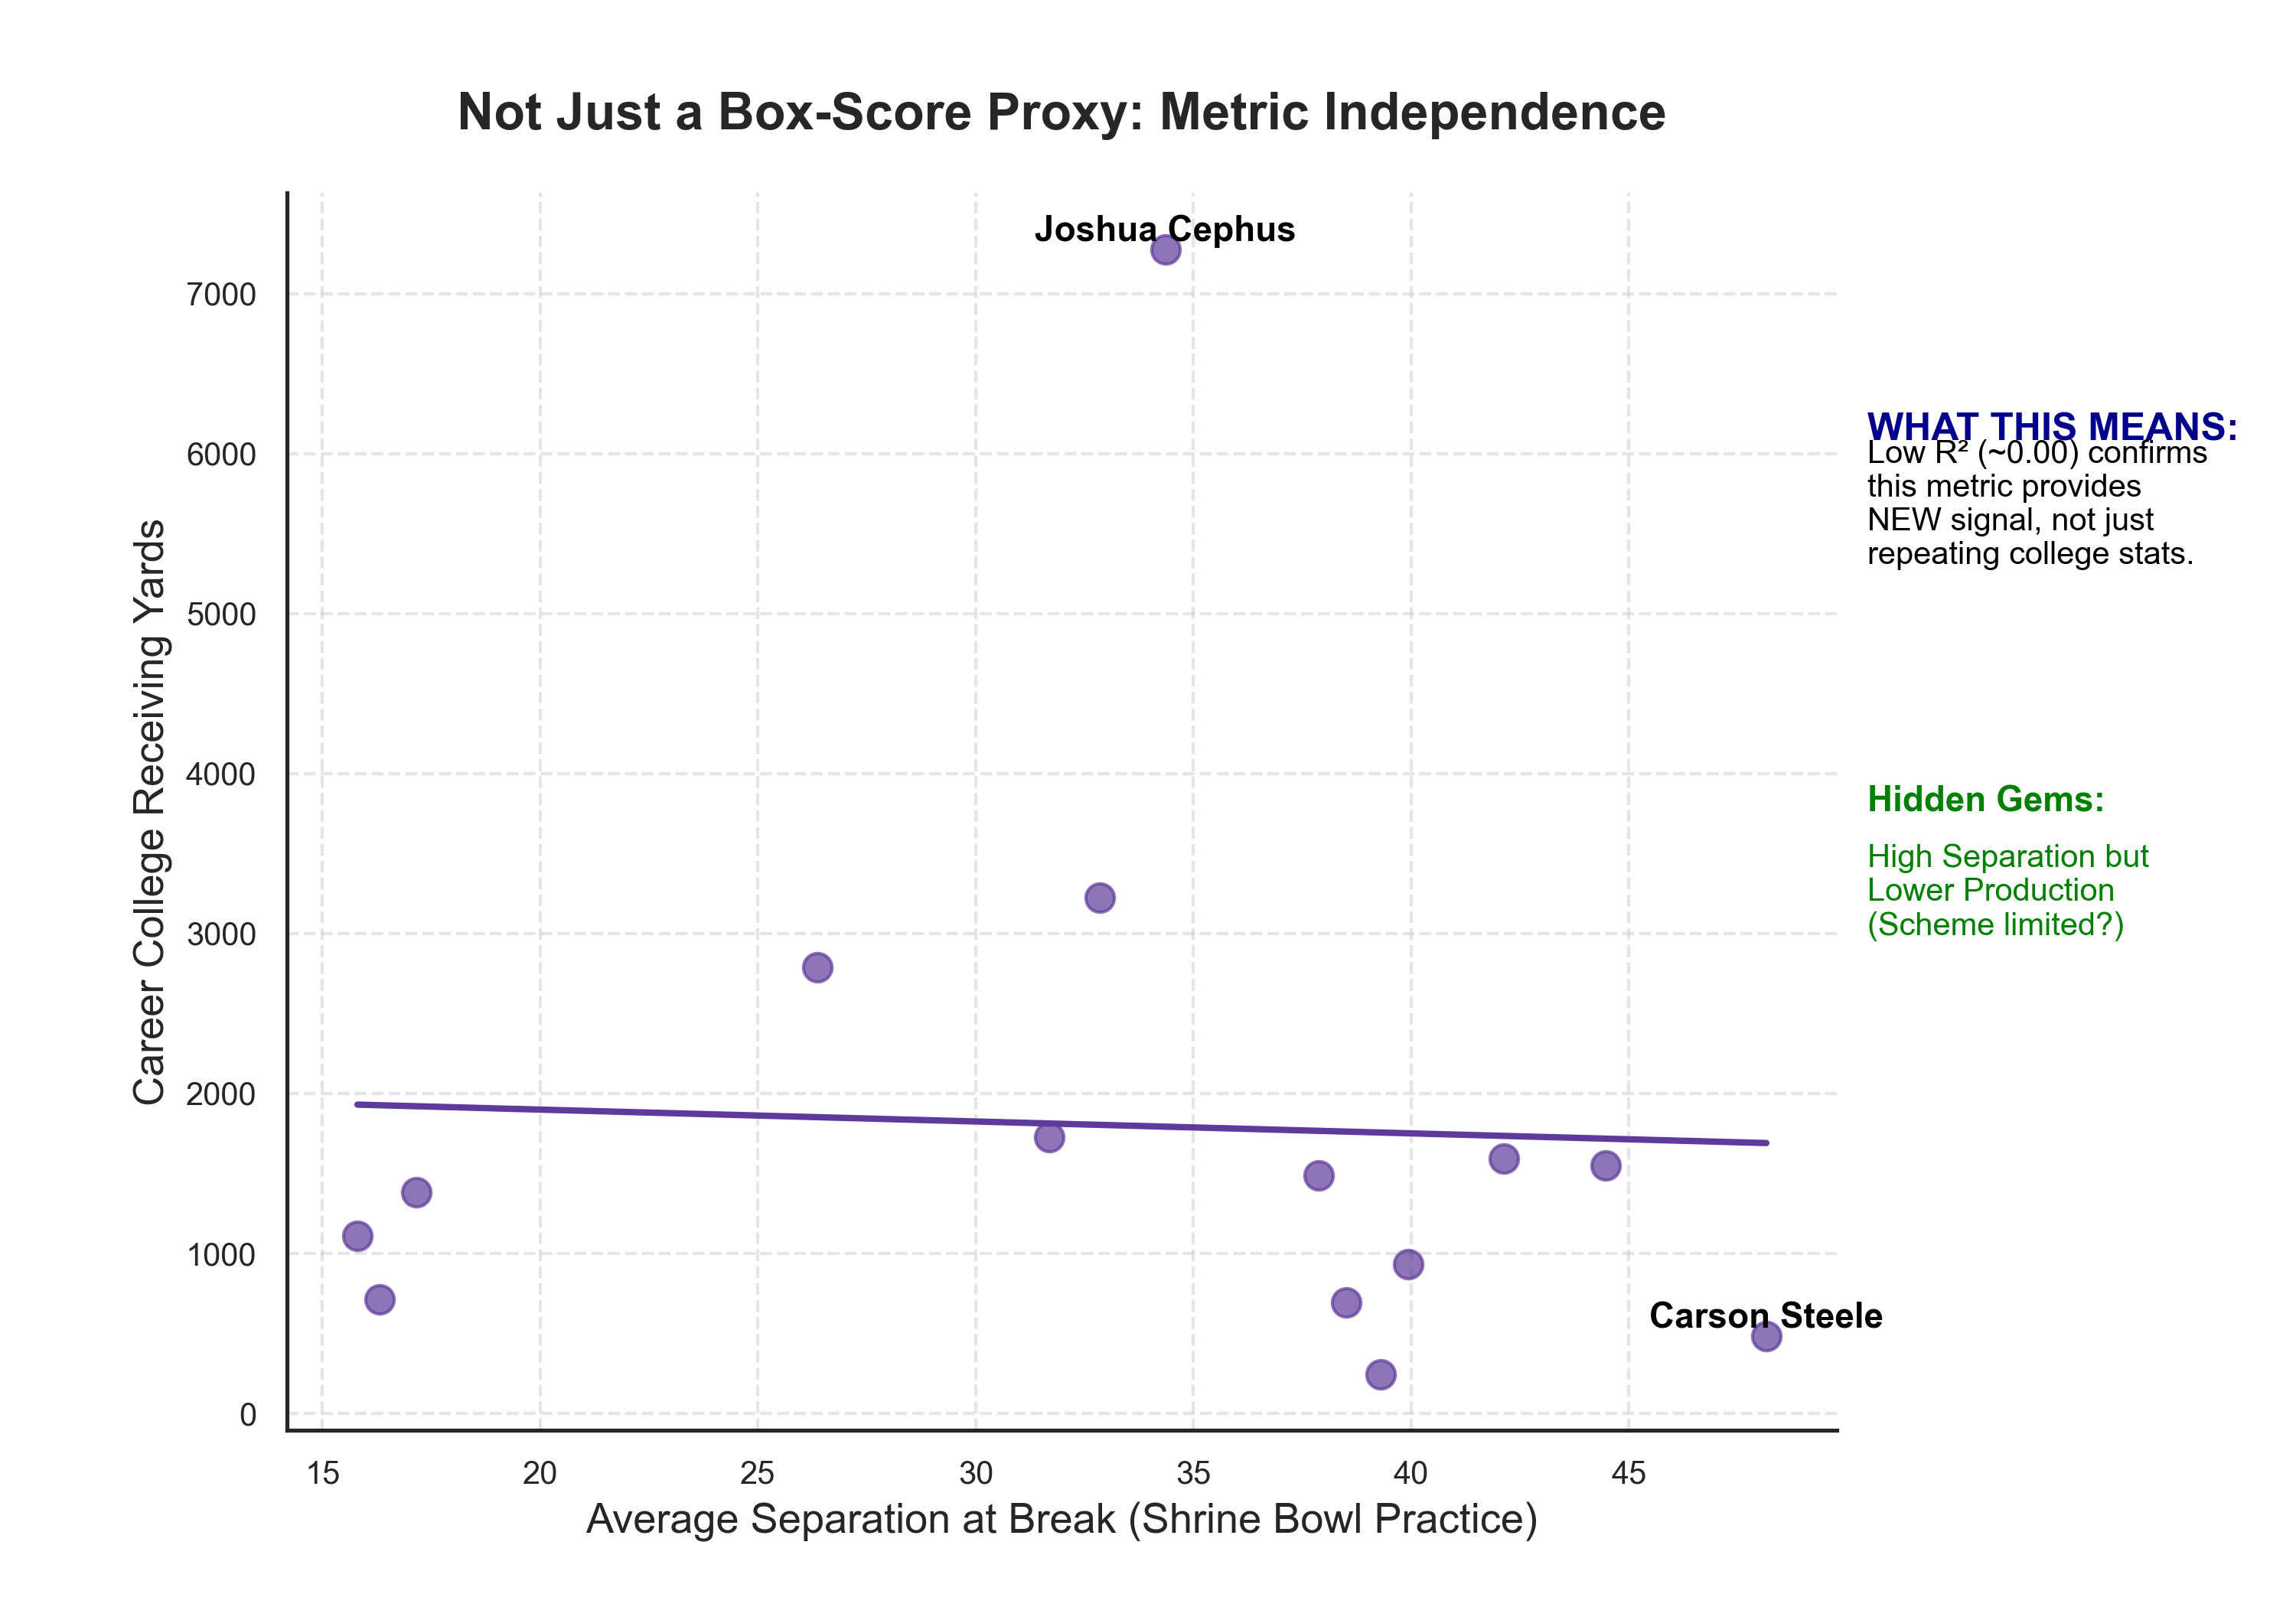
\includegraphics[width=\textwidth]{viz_correlation.png}
        
        \column{0.35\textwidth}
        \textbf{Fresh Intel:}
        \begin{itemize}
            \item \textbf{Unique Signal:} Low correlation ($R^2 \approx 0.04$) proves this metric captures specific 1-on-1 traits, independent of college production.
            \item \textbf{High Upside:} Identifies talent that may have been scheme-limited in college but is winning "The Moment" right now.
        \end{itemize}
    \end{columns}
\end{frame}

% Slide 9: Advanced Profiles (Stylistic Fit)
\begin{frame}{8. Player Profiling: "The Glue" vs "The Technicians"}
    \begin{columns}
        \column{0.48\textwidth}
        \centering
        \textbf{Defender Archetypes (Burst)}
        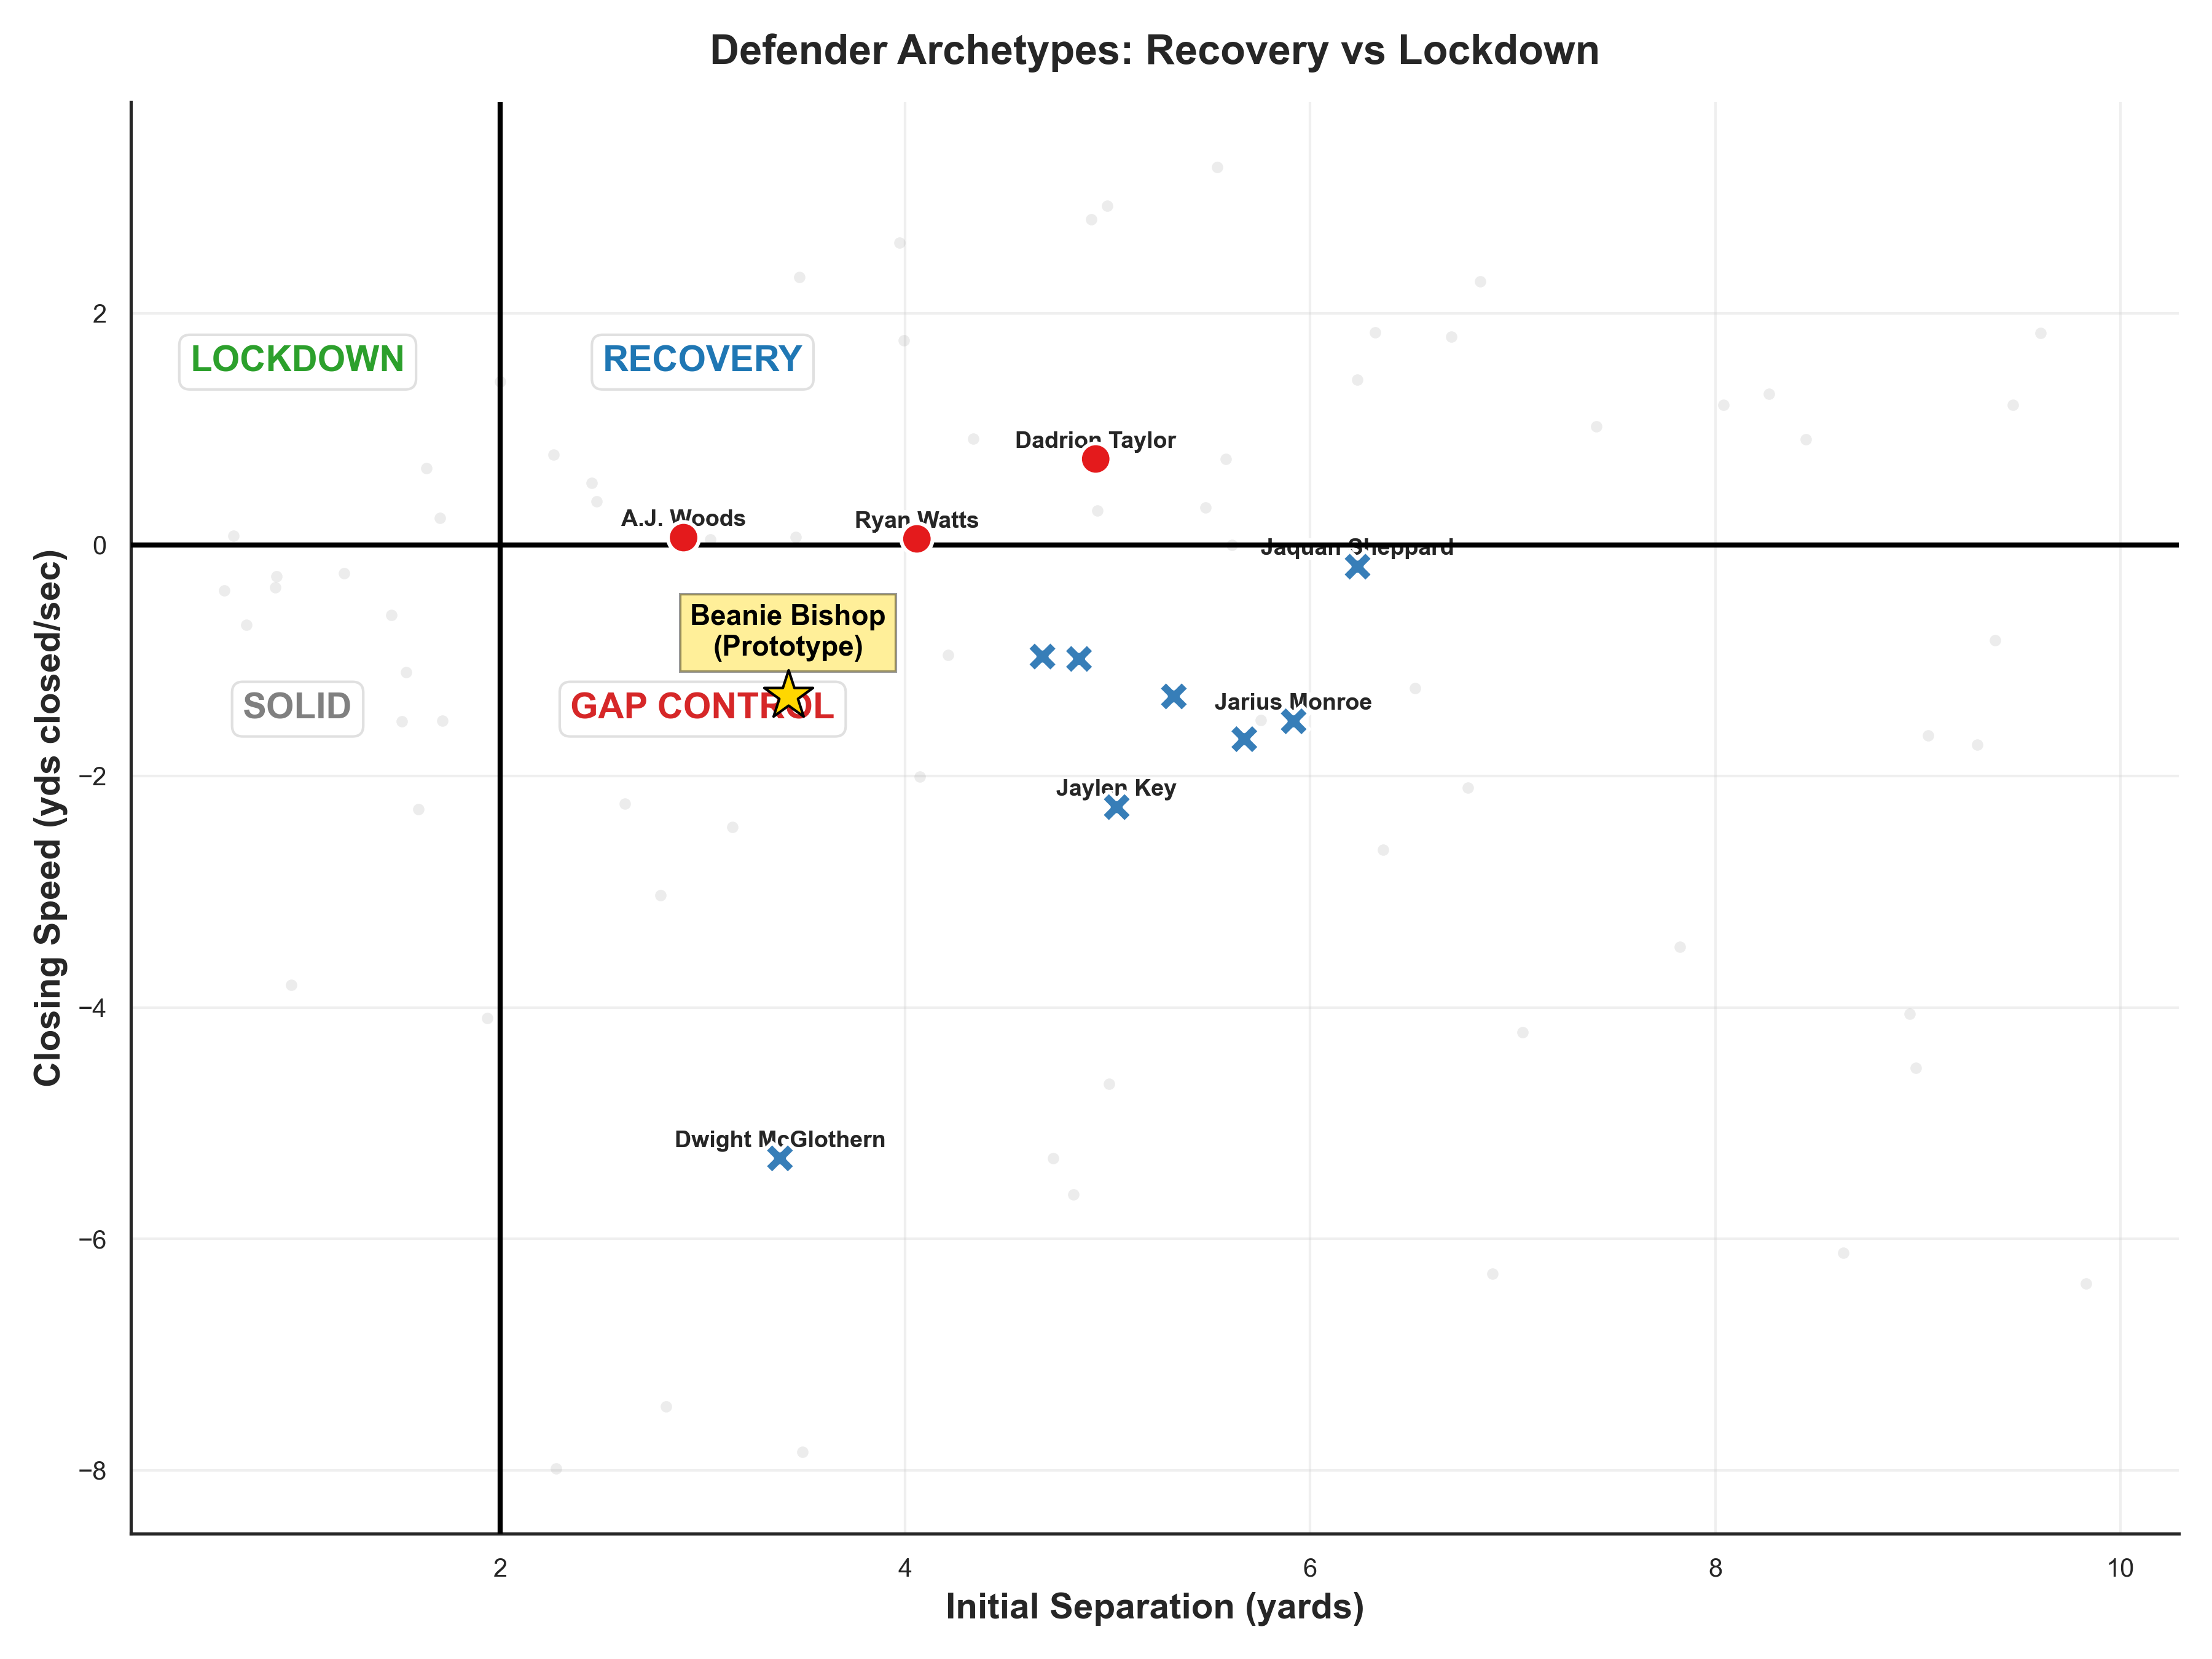
\includegraphics[width=\textwidth, height=3.8cm, keepaspectratio]{viz_burst.png}
        
        \column{0.48\textwidth}
        \centering
        \textbf{Receiver Profiles (Spider)}
        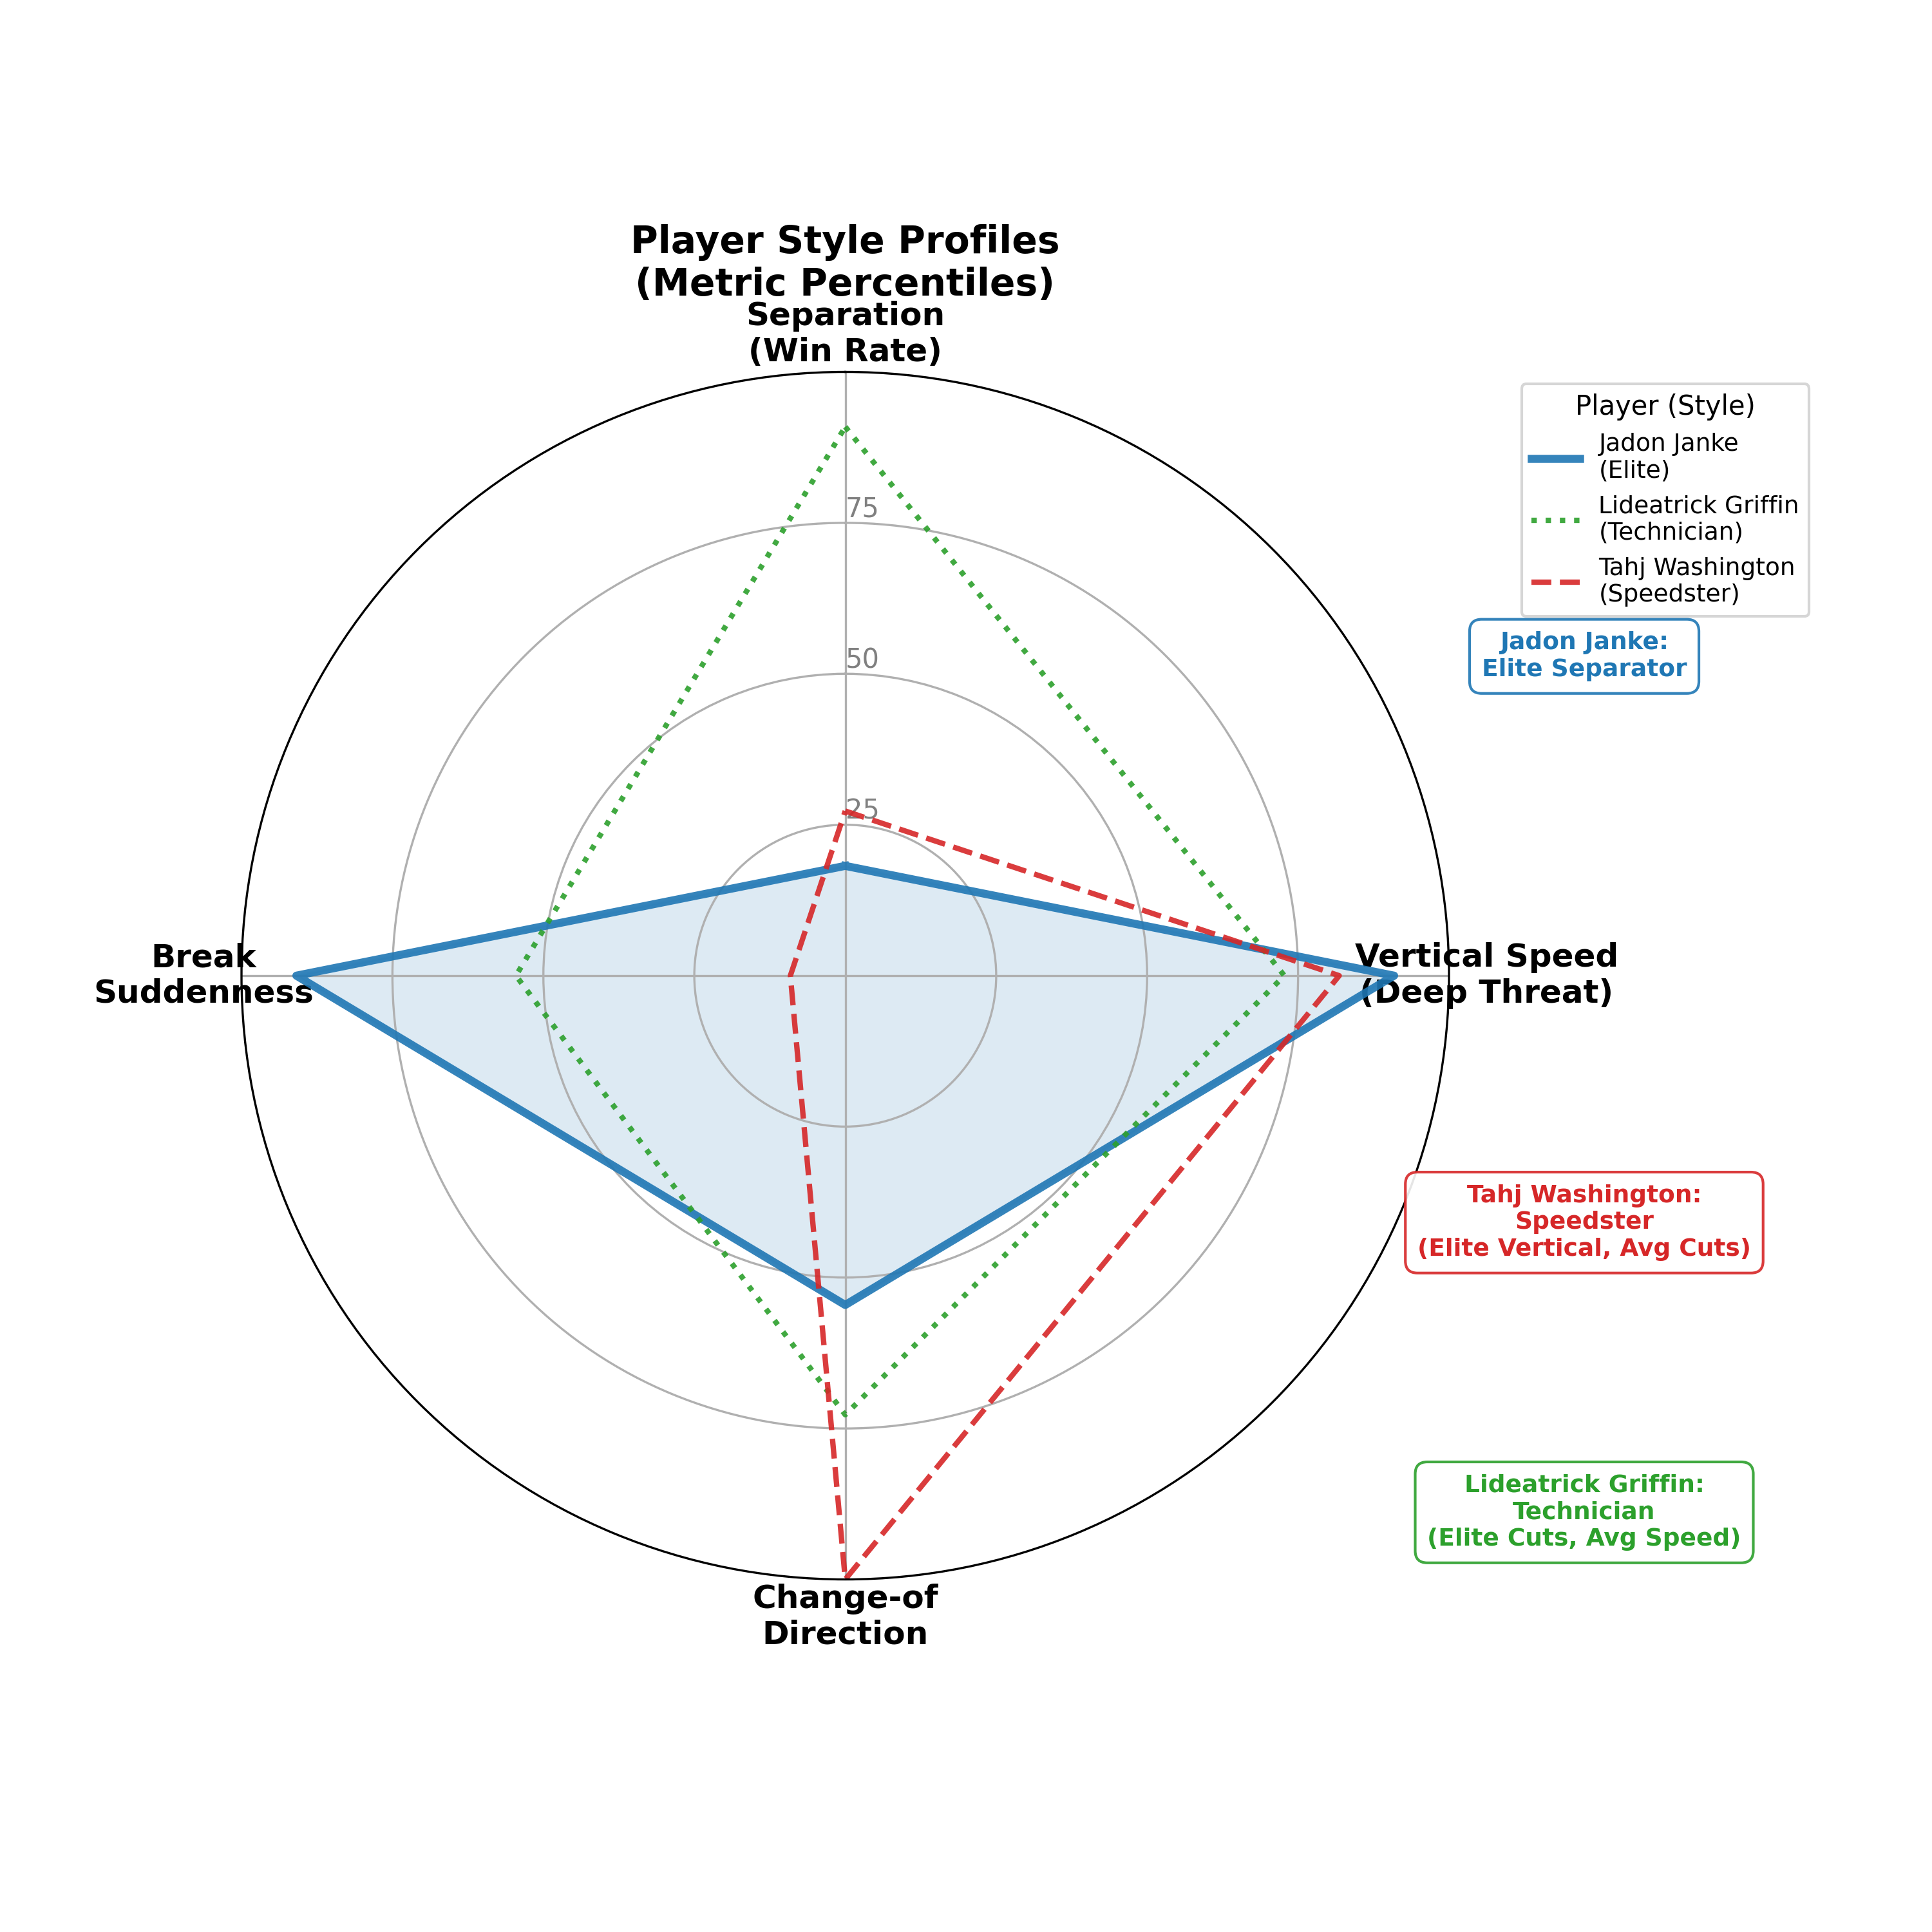
\includegraphics[width=\textwidth, height=3.8cm, keepaspectratio]{viz_spider.png}
    \end{columns}
    
    \vspace{0.1cm}
    \begin{block}{Scheme Fit Analysis}
        \footnotesize
        \begin{itemize}
            \item \textbf{Defenders (Left):} We cluster DBs by \textit{Reaction Latency} vs \textit{Closing Burst}. This identifies "Man-Match" corners vs "Zone" defenders.
            \item \textbf{Receivers (Right):} The Spider Chart identifies if a WR wins with \textit{Route Depth} (Deep Threat) or \textit{Break Angle} (Slot Weapon).
        \end{itemize}
    \end{block}
\end{frame}

% Slide 10: Conclusion
\begin{frame}{9. Conclusion \& Future Work}
    \begin{center}
        \huge \textbf{\textcolor{DarkBlue}{The Bottom Line}}
    \end{center}
    
    \vspace{0.3cm}
    \centering
    \large "We don't just see \textit{if} they are open. We measure \textbf{how} they got open."
    \vspace{0.3cm}

    \begin{columns}
        \column{0.5\textwidth}
        \begin{block}{For the Draft Room}
            Identify \textbf{Elite Separators} masked by poor QB play.
            \vspace{0.1cm}
            \textit{(Finding the next hidden gem)}
        \end{block}

        \column{0.5\textwidth}
        \begin{block}{For Pro Scouting}
            Find \textbf{"Eraser" DBs} who vanish space in less than 1 second.
            \vspace{0.1cm}
            \textit{(Finding the true lockdown corner)}
        \end{block}
    \end{columns}
    

    
    \vspace{0.8cm}
    \centering \Huge \textbf{\textcolor{AccentGold}{Thank You.}}
\end{frame}

\end{document}
